% Sablon pentru realizarea lucrarii de licenta, conform cu recomandarile
% din ghidul de redactare:
% - https://fmi.unibuc.ro/finalizare-studii/
% - https://drive.google.com/file/d/1xj9kZZgTkcKMJkMLRuoYRgLQ1O8CX0mv/view

% Multumiri lui Gabriel Majeri, acest sablon a fost creat pe baza
% codului sursa a lucrarii sale de licenta. 
% Codul sursa: https://github.com/GabrielMajeri/bachelors-thesis
% Website: https://www.gabrielmajeri.ro/
%
% Aceast sablon este licentiat sub Creative Commons Attribution 4.0 International License.

\documentclass[12pt, a4paper]{report}

% Suport pentru diacritice și alte simboluri
\usepackage{fontspec}
% Suport pentru mai multe limbi
\usepackage{polyglossia}
% \usepackage{blindtext}
\usepackage{caption}
% \counterwithout{figure}{chapter}
% Setează limba textului la română
\setdefaultlanguage{english}
\setcounter{secnumdepth}{3}
% Am nevoie de engleză pentru rezumat
\setotherlanguages{romanian}

% Indentează și primul paragraf al fiecărei noi secțiuni
\SetLanguageKeys{english}{indentfirst=true}

% Suport pentru diferite stiluri de ghilimele
\usepackage{csquotes}

\DeclareQuoteStyle{english}
  {\quotedblbase}
  {\textquotedblright}
  {\guillemotleft}
  {\guillemotright}

% Utilizează biblatex pentru referințe bibliografice
\usepackage[
    maxbibnames=50,
    sorting=nty
]{biblatex}

\addbibresource{bibliography.bib}

% Setează spațiere inter-linie la 1.5
\usepackage{setspace}
\onehalfspacing

% Modificarea geometriei paginii
\usepackage{geometry}

% Include funcțiile de grafică
\usepackage{graphicx}
% Încarcă imaginile din directorul `images`
\graphicspath{{./images/}}

% Listări de cod
\usepackage{listings}

% Linkuri interactive în PDF
\usepackage[
    colorlinks,
    linkcolor={black},
    menucolor={black},
    citecolor={black},
    urlcolor={blue}
]{hyperref}

% Simboluri matematice codificate Unicode
\usepackage[warnings-off={mathtools-colon,mathtools-overbracket}]{unicode-math}

% Comenzi matematice
\usepackage{amsmath}
\usepackage{mathtools}

% Formule matematice
\newcommand{\bigO}[1]{\symcal{O}\left(#1\right)}
\DeclarePairedDelimiter\abs{\lvert}{\rvert}

% Suport pentru rezumat în două limbi
% Bazat pe https://tex.stackexchange.com/a/70818
\newenvironment{abstractpage}
  {\cleardoublepage\vspace*{\fill}\thispagestyle{empty}}
  {\vfill\cleardoublepage}
\renewenvironment{abstract}[1]
  {\bigskip\selectlanguage{#1}%
   \begin{center}\bfseries\abstractname\end{center}}
  {\par\bigskip}

% Suport pentru anexe
\usepackage{appendix}

% Stiluri diferite de headere și footere
\usepackage{fancyhdr}

\usepackage{enumitem}

% Metadate
\title{\large Using Large Language Models in Translationese Classification}
\author{Baciu Daniel Mihai}

% Generează variabilele cu @
\makeatletter

\begin{document}

% Front matter
\cleardoublepage
\let\ps@plain

% Pagina de titlu
\begin{titlepage}

% Redu marginile
\newgeometry{top=2.5cm,left=2cm,right=2cm,bottom=1cm}

\begin{figure}[!htb]
    \centering
    \begin{minipage}{0.2\textwidth}
        
\includegraphics[width=\linewidth]{logo-ub.png}
    \end{minipage}
    \begin{minipage}{0.5\textwidth}
        \large
        \vspace{-0.35cm}
        \begin{center}
            \textbf{UNIVERSITY OF BUCHAREST}
        \end{center}
        \vspace{-0.45cm}
        \begin{center}
            \textbf{
                FACULTY OF \\
                MATHEMATICS \\
                AND \\
                COMPUTER SCIENCE
            }
        \end{center}
    \end{minipage}
    \begin{minipage}{0.2\textwidth}
        
\includegraphics[width=\linewidth]{logo-fmi.png}
    \end{minipage}
\end{figure}

\vspace{1.5cm}

\begin{center}
\textbf{COMPUTER SCIENCE}
\end{center}

\vspace{1cm}

\begin{center}
\Large \textbf{Bachelor Thesis}
\end{center}

\vspace{1cm}

\begin{center}
\huge \textbf{\MakeUppercase{\@title}}
\end{center}

\vspace{2cm}

\begin{center}
\large \textbf{Graduate \\ \@author}
\end{center}

\vspace{0.25cm}

\begin{center}
\large \textbf{Scientific coordinator \\ Lect. Dr. Dumitru Bogdan Costinel}
\end{center}

\vspace{1.5cm}

\begin{center}
\Large \textbf{Bucharest, June 2023}
\end{center}
\end{titlepage}
\restoregeometry
\newgeometry{
    margin=2.5cm
}

\fancypagestyle{main}{
  \fancyhf{}
  \renewcommand\headrulewidth{0pt}
  \fancyhead[C]{}
  \fancyfoot[C]{\thepage}
}

\addtocounter{page}{1}

% Rezumatul
\begin{abstractpage}

\begin{abstract}{english}

Translationese, the unique linguistic characteristics found in translated texts, has garnered awareness in the fields of natural language processing (NLP) and translation studies. The following paper investigates the use of BERT (Bidirectional Encoder Representations from Transformers) for translationese classification, capitalizing on its contextual language modelling capabilities. The methodology we proposed involves fine-tuning a pre-trained BERT model using a large annotated data set of translationese samples. The performance of the BERT-based classifier is assessed against state-of-the-art methods on a data set, showcasing its accuracy in accurately classifying translationese. The results demonstrate improvements over traditional feature-based approaches and other deep learning models. Furthermore, detailed analysis and visualization techniques shed light on the learned representations and highlight the distinctive features captured by BERT. This research contributes to the expanding body of knowledge in translationese classification and demonstrates the efficacy of BERT in this domain. The suggested methodology can be expanded to various NLP tasks, including stylistic analysis, authorship attribution, and text classification in different linguistic domains.
\end{abstract}

\begin{abstract}{romanian}

Acest studiu explorează utilizarea modelelor lingvistice extinse în clasificarea traducerilor. Termenul "translationese" se referă la caracteristicile și tiparele distinctive care apar în texte traduse. Ne concentrăm în mod specific pe utilizarea modelului BERT (Bidirectional Encoder Representations from Transformers) în detectarea translationese-ului. Lucrarea începe cu o introducere care prezintă contextul și problema de cercetare. Apoi, efectuăm o revizuire a lucrărilor relevante din domeniu. În secțiunea preliminară, oferim o prezentare generală a Transformatorilor, modelului BERT și bibliotecii Hugging Face, care sunt componente esențiale pentru abordarea noastră. Ulterior, detaliem modelul propus pentru detectarea traducerilor, inclusiv arhitectura și variantele acestuia. Secțiunea dedicată studiului experimental discută datele utilizate și prezintă rezultatele obținute prin abordarea noastră. În final, concluzia rezumă descoperirile, evidențiază limitele studiului nostru și sugerează direcții potențiale pentru cercetări viitoare.
\end{abstract}

% \begin{abstract}{english}

% Translationese, the unique linguistic characteristics found in translated texts, has garnered significant attention in the fields of natural language processing (NLP) and translation studies. This paper investigates the use of BERT (Bidirectional Encoder Representations from Transformers) for translationese classification, capitalizing on its contextual language modelling capabilities. The proposed methodology involves fine-tuning a pre-trained BERT model using a large annotated dataset of translationese samples. The performance of the BERT-based classifier is evaluated against state-of-the-art methods on a dataset, showcasing its accuracy in accurately classifying translationese. The results demonstrate significant improvements over traditional feature-based approaches and other deep learning models. Furthermore, detailed analysis and visualization techniques shed light on the learned representations and highlight the distinctive features captured by BERT. This research contributes to the expanding body of knowledge in translationese classification and demonstrates the efficacy of BERT in this domain. The proposed methodology can be extended to various NLP tasks, including stylistic analysis, authorship attribution, and text classification in different linguistic domains.

% \end{abstract}

% \begin{abstract}{romana}
% Rezumat:
% Traducerea, fenomenul lingvistic care implică artefacte și particularități specifice textelor traduse, a atras o atenție semnificativă în domeniul procesării limbajului natural (PLN) și al studiilor de traducere. Detectarea și clasificarea fenomenului de "traducere" poate oferi înțelegere asupra procesului de traducere și poate fi folosită în diverse aplicații de PLN. Această lucrare explorează aplicarea modelului BERT (Bidirectional Encoder Representations from Transformers) în clasificarea textelor în limba traducerilor, profitând de capacitatea sa de modelare a limbajului în context. Propunem o metodologie care implică ajustarea unui model BERT pre-antrenat pe un set mare de date etichetate care conțin exemple de text în limba traducerilor. Evaluăm performanța clasificatorului bazat pe BERT în comparație cu metodele curente de ultimă generație pe mai multe seturi de date și demonstrăm eficacitatea sa în clasificarea exactă a textelor în limba traducerilor. Rezultatele arată că BERT obține îmbunătățiri semnificative în acuratețea clasificării, depășind abordările tradiționale bazate pe caracteristici și alte modele de învățare profundă. În plus, efectuăm analize detaliate și tehnici de vizualizare pentru a obține înțelegere asupra reprezentărilor învățate și evidențiem caracteristicile discriminante capturate de BERT. Descoperirile noastre contribuie la corpul tot mai mare de cercetare în clasificarea textelor în limba traducerilor și evidențiază eficacitatea modelului BERT în acest domeniu. Metodologia propusă poate fi extinsă la diverse sarcini de PLN care implică analiza stilistică, atribuirea autorului și clasificarea textelor în alte domenii lingvistice.

% \end{abstract}

\end{abstractpage}

\tableofcontents

% Main matter
\cleardoublepage
\pagestyle{main}
\let\ps@plain\ps@main

\chapter{Introduction}

As we further advance into the age of artificial intelligence, an array of debates have emerged, ranging from the ethical implications of AI to its potential to replace human labour in various sectors. One area of AI that has been at the forefront of these discussions is text generation software. These tools, capable of creating content nearly indistinguishable from human writing, have been met with acclaim and criticism. Yet, while these debates continue, one branch of AI remains less contentious but equally compelling – translation software.

The advent of powerful, large language models has transformed various aspects of the natural language processing (NLP) field, including the realm of Translationese Classification \cite{2_translationese}. This area of work is dedicated to studying and analysing translated texts, often referred to as 'translationese,' due to their distinctive characteristics compared to original, non-translated compositions. The study of translationese, despite its academic actuality and relevance, is yet to be exhaustively explored, especially with respect to leveraging modern language models in the process \cite{2_4_translationese}. 

This thesis, titled "Using Large Language Models in Translationese Classification", will contribute to filling this research gap.
Our aim is to contribute to the growing body of knowledge that seeks to improve the accuracy and efficiency of translation software.

There are many factors that will further increase the usage of the translation software in the following decades and thus create higher demand for better language processing models. Among these factors, we can observe the widespread usage of the internet in the 21st century alongside an increasingly multicultural and multilingual work and life environment. These advancements will most likely lead to a society where one main language is used more than the others, but also real-time cross-lingual conversations might become a common occurrence with the help of translation technology.

\section{Background}

Translationese classification, the process of discerning translated texts from native ones, has increased in importance in recent years because of the need for accurate communication, the limitations of automated translation tools, the significance of cultural appropriateness, a growing demand for the global reach of content, and the importance of preserving native languages. As the world becomes more interconnected and multilingual, the demand for translation, and thus, the need for its quality assessment and detection has been rising in numerous fields and industries.

Machine translation (MT)\cite{background}, the usage of machines in the scope of text translation, has been an area of extensive research for over 70 years, evolving with the advent of artificial intelligence and deep learning systems. In an increasingly globalised context, language barriers can limit access to vast amounts of daily information. Machine translation is seen as a potential solution, providing multilingual access to various types of audiences. It also plays a critical role in indirect translations where texts are translated to a target language via a mediating language, helping to reduce operating costs in an ever-increasing multicultural and multilingual world, as well as helping to manage language combinations that are not as common.

Translationese classification, thus, has become a necessary tool to assess the quality and reliability of machine translations, comparing them to human translations. As the translation process involves various strategies, techniques, and equivalence types, identifying translationese becomes an intricate task. This identification has implications in multiple areas, such as forensic linguistics, where identifying the authorship of translated texts is crucial, and legal fields, where detecting instances of plagiarism or copyright infringement is necessary.

Machine learning methods have been applied for translationese classification and have been shown to outperform traditional manual feature engineering approaches. These models can better capture the intricate linguistic patterns and the influences of translation strategies, cultural factors, and language variations. For instance, models such as BERT have demonstrated superior performance in translationese classification tasks, improving upon the limitations of traditional feature engineering methods.

\section{Research Problem}

Research in the field of machine translation (MT) has long been grappling with the task of improving translation accuracy. Traditional MT systems face numerous challenges such as the correct resolution of written text and communication ambiguities in the source and expressing its intended meaning in a concise and easy-to-read manner. Maintaining consistency in domain-specific translations is also a major concern in MT applications.

Recently, Large Language Models (LLMs), such as GPT-4, have demonstrated outstanding performance in natural language processing (NLP) tasks, which includes machine translation. Despite their impressive results, the current research reveals that LLMs perform relatively poorly at the segment level, indicating room for improvement.

A crucial aspect often overlooked in conventional MT systems is the preparatory steps taken by human translators. Professional translators analyze key features of a text such as keywords, topics, and example sentences before translating. Traditional MT systems, which focus primarily on direct source-to-target mapping, need to pay more attention to these preparatory steps. Such steps resemble the procedures of feature engineering in machine learning, which requires creating meaningful variables that capture underlying patterns in data.

This research problem highlights two primary areas. Firstly, it underscores the limitations of conventional feature engineering techniques in effectively capturing the unique patterns, referred to as translationese, in the translated text. Secondly, it underscores the potential of LLMs to improve translation detection accuracy.

The paper aims to tighten te gap between current literature and a need for more robust and scalable approaches to translationese classification. The main objectives of this investigation are:

Firstly, to investigate the limitations of conventional feature engineering procedural approaches in capturing translationese patterns, thereby better defining the problem at hand.

Secondly, to explore the potential of LLMs in enhancing the accuracy of translation detection, focusing on the possibility of using these models in a novel way to overcome the identified limitations of traditional feature engineering.

The significance of this research stems from the potential applications of accurate translation detection in diverse bodies of work such as academic research, international relations, and machine translation technology development.

The research problem of this study is centred around the question: How can we make better use of the capabilities of large language models to better translation detection accuracy? The proposed research seeks to shed light on the problems, aiming to advance the field of machine translation research.


\section{Thesis Structure}


The proposed structure of this thesis is designed to be easy to read and understand. It begins with the title page, followed by the abstract, which is a brief summary of the study, including the topic under study, the methodology used, and the main results and findings.

Chapter 1 provides the reason why the chosen topic is important to study, and offers contextual information about the topic, specifically, translationese and ways to enhance systems related to it.

Chapter 2 is made up of a broad presentation of the already published literature on the subject. It examines current approaches' strengths and weaknesses and identifies existing research gaps.

Chapter 3 consists of the preliminary study used to understand the theory concerning software related to the topic at hand. The section explores a detailed analysis of Transformers, BERT and Hugging Face.

Chapter 4 describes the steps used to apply the theoretical knowledge previously gathered into a practical experiment. The material includes a detailed description of the models and layers used, calculus formulas, and mechanisms behind them.

Chapter 5 presents the experimental research undertaken in detail. It provides a description of how the study was carried out, data exploration, pre-processing procedures, as well as results for two experiments.

Chapter 6 analyzes the data collected in the study and draws conclusions based on the found information. Furthermore, it breaks down the meanings of the conclusions for the broader field of study and its future, as well as provides recommendations.

Lastly, in the bibliography we included all the references cited throughout the thesis, offering a comprehensive list of all the sources consulted during the research process.

\chapter{Related Work}

The second chapter of the paper "Using Large Language Models in Translationese Classification" is dedicated to the exploration and analysis of related work in translationese classification. A comprehensive literature review is provided, presenting existing approaches, highlighting their strengths and weaknesses, and identifying the gaps in the current research.

\section{Overview of Translationese Classification Approaches}

The study of 'translationese' investigates the unique linguistic traits that distinguish translated texts from non-translated ones. Various computational and machine-learning methods have been employed for this task. In this overview, we discuss some of the prominent approaches to translationese classification, highlighting their strengths, limitations, and effectiveness.


Rule-based methods rely on specific linguistic patterns or heuristics to identify translationese. These approaches are often grounded in linguistic theories and observations made in translation studies. For example, certain translation-specific features like the overuse of function words, specific morphosyntactic categories, personal pronouns, and adverbs have been used to recognize translated text. Rule-based methods have the advantage of providing interpretable results since the rules or patterns can often be related to specific linguistic phenomena. However, these methods may need help to generalise due to the diversity and variability in translationese.

Statistical methods utilize various language models or statistical measures to distinguish translations from native texts. Support Vector Machines (SVMs), for instance, have been employed with success in recognizing translated text, achieving high accuracy and precision. They often use features such as the distribution of function words and morphosyntactic categories and show significant improvement when adding simplification features. However, traditional statistical methods often rely on manual feature engineering, which can be time-consuming and require linguistic expertise.

Machine learning, particularly neural networks, has shown promise in translationese classification. These methods often outperform traditional manual feature engineering-based approaches, such as SVMs, by learning salient features directly from the data. Neural architectures, including BERT, have shown superior performance in this task. For example, using BERT representations with SVM classifiers yields results comparable to those of the best BERT classifiers.

Moreover, machine learning techniques allow for the investigation of translationese in various contexts, such as human translations, simultaneous interpreting, or machine translations. They detect translationese in non-invaside ways and compare it across different translation modalities. However, a limitation of neural models is their 'black-box' nature, which often makes the learned features less interpretable.

The field is gradually moving towards feature-learning-based approaches and neural architectures, which do not require manual feature engineering. Although neural models have been less explored for this task, recent advancements in language models suggest a promising direction for translationese classification. For example, pre-trained neural word embeddings and various end-to-end neural architectures can be employed in both monolingual and multilingual contexts.

While there are several effective methods for translationese classification, each approach comes with its own strengths and limitations. The task remains challenging due to the complexities and variations in translationese. Nevertheless, the advancements in machine learning, particularly neural networks, offer promising directions for future research.


\section{Linguistic Features for Translationese Classification}

Numerous studies have examined various linguistic aspects, such as lexical, syntactic, semantic, and stylistic features, to classify and distinguish translationese.

Lexical features primarily focus on word frequencies and n-gram models. Word frequency is a commonly used linguistic feature in translationese studies as it can help identify the occurrence and repetition of words in translated texts compared to original ones. N-gram models, which are sequences of n words, are another critical feature used to characterize translationese. The use of n-gram models, especially bigrams, trigrams, and 4-grams, in part-of-speech tags has been successfully applied to investigate genre and method variation in a translation corpus.

Syntactic features involve the grammatical structure of sentences. A common method used to extract syntactic features is parsing, which can generate parse trees to represent sentence structure. Part-of-speech tags and syntactic parse trees are used to classify and differentiate between translations and native texts.

Semantic features relate to the meaning of words and sentences. One semantic feature used in translationese classification is semantic representations, which involve capturing the meaning of words and sentences in a computable form. Although the literature provided does not mention specific semantic features used in translationese classification, previous research has shown that certain linguistic representations derived by Natural Language Processing (NLP) techniques, such as word senses and syntactic relations, have been observed to be ineffective in improving document retrieval and text categorization.

Stylistic features in translationese are often related to specific choices made by translators, potentially influenced by their source language, which can contribute to the unique style of translated texts.

The effectiveness of these features in differentiating translations from native texts is examined along with their limitations. Features specific to translations or those occurring with significantly variable frequency in translations than in originals are effective in distinguishing translated texts.

However, challenges related to feature selection, feature engineering, and the robustness of these features across different languages and translation domains remain. One major limitation is that the choice of features can be heavily influenced by the type of texts under investigation. For instance, certain features may be more prominent in literary translations as compared to technical or scientific translations.

Moreover, the effect of the translator's individual style, the translation method, and the period during which the translation was made can also significantly affect the appearance of translationese features. Consequently, more research is required to ensure the generalizability of these features across different translation corpora and contexts.

Additionally, computational methods used for feature extraction and classification also have limitations. Many studies rely on supervised machine learning methods, which require labelled data for training. This requirement may limit the scalability of these methods since labelling data can be time-consuming and requires expert knowledge. Furthermore, the performance of these methods can be affected by issues such as class imbalance and overfitting.


\section{Feature Engineering Techniques}

An important crucial step in machine learning and natural language processing (NLP) applications, including translationese classification is represented by feature engineering. This process is focused on the creation of new features or the adjustment of already existing ones, with the purpose of model performance improvement. The objective is to extract the most informative and relevant attributes that can improve the predictive power of the model, thereby enhancing the classification results.

In the context of translationese classification, feature engineering can involve extracting linguistic attributes such as the syntactic, semantic, and stylistic properties of the text. This is often done using hand-picked linguistic features which have been traditionally utilized for identifying translated and non-translated texts.

Preprocessing forms the first stage of feature engineering. Text normalization methods such as tokenization, stop-word removal, and stemming are widespread techniques. Tokenization breaks down the text into smaller parts like words or sentences. Stop-word removal excludes common words like 'is', 'the', 'and', which do not carry much meaningful information for analysis. Stemming reduces words to their root form.

Feature selection, the next step, is used to identify the most informative features for classification. Methods like chi-square or mutual information can be used to quantify the bridge between every input variable and the target variable. Features that exhibit strong correlation with the target variable are usually selected.

In cases where feature vectors have a high dimensionality, dimensionality reduction techniques like PCA or LDA can be applied. These methods reduce the dimensionality of feature vectors without losing significant information, making the data more manageable and reducing computational costs.

Feature engineering can significantly enhance the performance of translationese classification. However, there is a trade-off between the complexity of feature engineering and the computational cost or interpretability of the models. Furthermore, one of the challenges is to ensure that the engineered features are generalizable across different translation domains or languages.

While feature engineering is crucial when it comes to translationese classification, care must be taken to select and engineer features that will not only improve classification performance but also maintain generalizability across different contexts. It is also important to balance the complexity of the features and the computational and interpretability costs associated with them.



\section{Previous Approaches using Large Language Models}

The past decade has seen a dramatic shift in the field of machine learning, with the advent and proliferation of large language models like Transformers, BERT, GPT, and their variants. These models have been applied across numerous NLP tasks, and this text specifically focuses on their use in translationese classification.

Large language models' potential for translationese classification was initially recognized due to their robustness in capturing complex linguistic contexts. Traditional methods, based mostly on rule-based algorithms and shallow learning models, struggled with the complexity and variability inherent in this task. They were largely limited by their inability to handle long-range dependencies and the vast number of language-specific nuances.

The first significant milestone was the adoption of Transformer models in translationese classification. These models, introduced by Vaswani et al. in 2017 \cite{attention}, were revolutionary due to their unique architecture that permitted the model to attend to any part of the input sequence, thereby effectively capturing long-range dependencies. Many studies leveraging Transformers showed a noticeable improvement in accuracy and robustness compared to traditional methods.

BERT (Bidirectional Encoder Representations from Transformers) further improved upon the Transformer architecture by pre-training the model on a large corpus of text and then fine-tuning it for specific tasks, such as translationese classification. This approach provided the model with a more nuanced understanding of language, contributing to better performance. The robustness of BERT was evidenced in a 2020 study \cite{DBLPewfiovncoi} that demonstrated its ability to excel in multi-lingual and domain-specific settings.

Subsequently, studies started utilizing GPT-like models, which, unlike BERT, are autoregressive and generate outputs one token at a time. Although primarily used for text generation, GPT-like models' remarkable ability to handle language-specific phenomena made them suitable for translationese classification. The application of GPT-like models to this task and their subsequent success was a testament to the models' flexibility and adaptability.

Despite the strides made by large language models, there have been challenges. The interpretability of these models has been a significant concern due to their black-box nature. Further, the trade-off between accuracy and computational resources is often a limiting factor, given that large language models require substantial computational power and storage.

The use of large language models in translationese classification has transformed the field, providing high accuracy and robustness against varied linguistic phenomena. Despite their challenges, their ability to capture complex language semantics and long-range dependencies, along with their adaptability to different languages and domains, ensures their continued relevance in translationese classification studies. Future work will likely focus on improving the model's' interpretability and efficiency.


\section{Summary and Identified Gaps}

The extensive review of the literature presented in the previous sections has underscored the rich and multidimensional landscape of translationese classification. Through various studies, different approaches have been utilized to tackle this challenging task, with the common goal of enhancing the understanding of the complexities and subtleties of the translated text.

Among the reviewed approaches, the utilization of large language models, such as Transformers or BERT\cite{BERT}, has emerged as a promising path. These models have demonstrated a strong capacity to capture contextual and semantic information, which is paramount in the field of translationese classification. Furthermore, large language models have shown to be effective in identifying long-range dependencies, a key feature in analyzing the structure and composition of the translated text.

Despite the promising results achieved by large language models in translationese classification \cite{xjsdhchuc3oiqwe}, our review identified several areas that have been inadequately addressed in previous research. These gaps in the literature provide us with the opportunity to expand and refine the existing approaches, thus propelling further advancements in the field.

Firstly, there is a noticeable gap in the exploration of translation errors across different literary genres. While several studies have focused on specific types of texts, such as newspapers and legal documents, the comprehensive analysis of translation errors across a variety of genres remains an area ripe for exploration. The ability of large language models to adapt to different languages and domains makes them particularly suited to address this gap.

Secondly, the issue of interpretability of large language models remains largely unaddressed. While these models have excelled in terms of accuracy, their "black box" nature poses a significant challenge. Developing methods that allow better interpretability of these models would not only improve our understanding of how these models work but also enhance our confidence in their results.

Thirdly, the trade-off between accuracy and computational resources is another area that has been insufficiently explored in previous studies. With the increasing complexity and size of large language models, the computational cost of utilizing these models is a significant consideration. Future research should focus on strategies to optimize this trade-off.

In light of these identified gaps, the subsequent chapters will present an approach that leverages the strengths of large language models to advance the field of translationese classification. The proposed approach aims to address the aforementioned gaps, with a particular emphasis on improving the interpretability of these models and optimizing the trade-off between accuracy and computational resources.




\chapter{Preliminary}

\section{Transformers}

Methodologies like Recurrent Neural Networks, Long Short-Term Memory, and Gated Recurrent Neural Networks have solidified their position as cutting-edge techniques in the field of sequence modeling and transduction challenges. Particularly in the areas of language modeling and machine translation is this apparent. Through several experiments, researchers have consistently pushed the limits of encoder-decoder structures and recurrent language models.


The symbolic positions of input and output sequences have traditionally been used as the foundation for recurrent models' calculations. These models create a series of hidden states denoted as $h_t$ that are influenced by the input at location t and the preceding hidden state $h_{t-1}$ by mapping these positions to computational time steps. Due to their innately sequential character, they are difficult to parallelize during training, particularly when dealing with longer sequences when memory constraints prevent batching across cases.

However, efforts have been made to increase computing efficiency using strategies such as conditional computation and factorization tricks. In some instances, the model performance has improved as a result of these developments. However, sequential computation continues to present a fundamental issue.


In an endeavor to minimize sequential computation, numerous theoretical frameworks have been developed, including the Extended Neural GPU, ByteNet, and ConvS2S. These frameworks share a common foundation centered around CNNs. Such models can compute hidden representations over all output and input places in simultaneously. Within these models, the computational complexity for establishing connections between any two arbitrary input or output locations follows a linear scaling pattern for ConvS2S and a logarithmic scaling pattern for ByteNet. The specific scaling behavior is determined by the distance between the respective positions being considered. When determining dependencies between distant sites, this scaling provides a more challenging task. The Transformer model, on the other hand, simplifies this scaling to a fixed set of actions. Despite the drawback of a reduced effective resolution caused by the averaging of attention-weighted positions, the utilization of Multi-Head Attention is employed as a countermeasure.

The Transformer model holds a unique distinction as the pioneering transduction model that exclusively employs self-attention methods to perform computations on its output and input representations, doing away with the requirement for sequence-aligned RNNs or convolutions. The Transformer model will be thoroughly described, the rationale for self-attention will be explained, and its comparative advantages over other models will be covered in the parts that follow.


\subsection{Model Architecture}
Modern neural designs for sequence transduction typically use encoder-decoder architectures. Within this particular configuration, the encoder is responsible for mapping a sequence of continuous representations, denoted as $(z_1,..., z_n)$, into a sequence of symbol representations, represented as $(x_1,..., x_n)$. Subsequently, the decoder generates an output sequence, $(y_1,..., y_m)$, iteratively, utilizing the information derived from these continuous representations. The model operates in an auto-regressive manner, incorporating the output of preceding symbols as additional input to generate the subsequent symbol at each step.

\begin{figure}[!h]
    \centering
    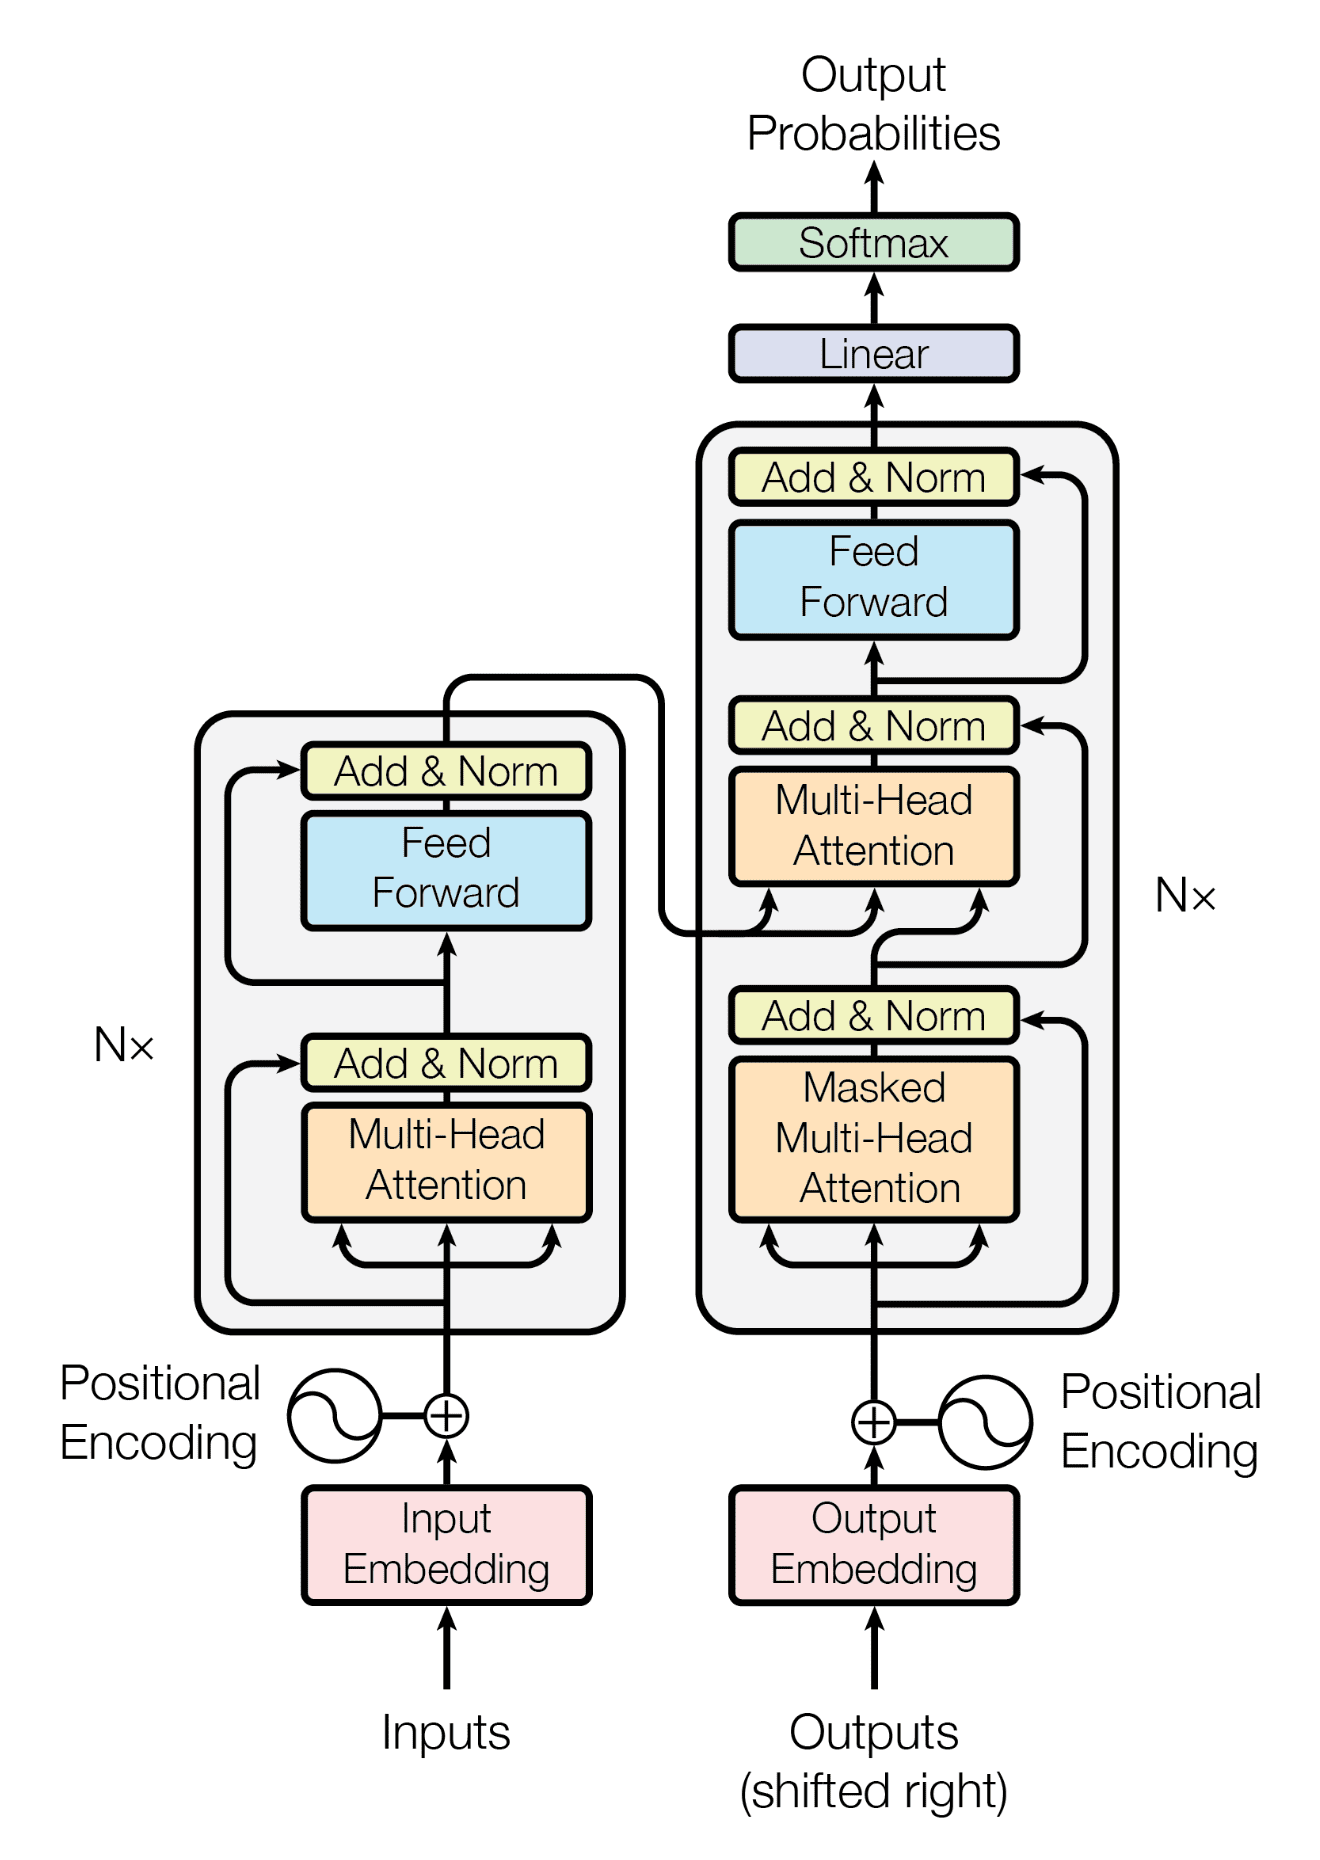
\includegraphics[height=10cm]{attention_research_1.png}
    \label{fig:transformer}
    \caption{Architecture of Transformer\cite{attention}}
\end{figure}

\subsection{Encoder and Decoder}

The architecture of the encoder comprises six homogeneous layers, wherein each layer encompasses two distinct sublayers. The initial sublayer implements a multi-head self-attention mechanism, while the subsequent sublayer employs a positionally entirely connected feed-forward network. Residual connections and layer normalization are put in an application for each sublayer. Consequently, the results of each sublayer are computed as LayerNorm(x + Sublayer(x)), where Sublayer(x) represents the function performed independently by each sublayer. To accommodate these residual connections, all sublayers and embedding layers in the model produce outputs with a dimensionality of $d_{model}$ = 512.

Components of Encoder : 

\begin{enumerate}
   \item Self-Attention Mechanism:
   \begin{enumerate}
        \item Scaled dot-product attention, also known as self-attention, enables the model to selectively centre around particular input sequence chunks. It determines a weighted sum of values (V) by assessing how similar the query (Q), key (K), and value vectors are to one another.
         A number of attention heads are identifiable in each encoder layer, allowing for the capturing of various dependencies and interactions within the sequence.
        
         \item Self-attention uses the Q and K dot product to calculate attention ratings, which are then scaled and normalized using softmax. When calculating the output, these scores are employed to account for the corresponding values.
         \item The encoder effectively captures long-range relationships and accounts for the contextual relevance of each token inside the sequence by using this attention method.


    \end{enumerate}
    
   \item Feed-Forward Neural Network:
    \begin{enumerate}
        \item The output then goes through extra processing through the FFN after the self-attention stage.

        \item A non-linear activation function, similar to ReLU, separates two linear transformations in the FFN.

        \item This network improves the encoder's capacity to detect complex relationships and patterns across distinct sequence segments.


    \end{enumerate}

   \item The Transformer model's architecture includes both layer normalization and residual connections:
    start the enumerationitem The outputs of each sub-layer are normalized using layer normalization after the self-attention mechanism and the feed-forward network.
\begin{enumerate}
        \item Additionally, residual connections are utilized to preserve data from earlier layers and lessen the difficulties associated with the vanishing gradient problem during training.

    \end{enumerate}

    \item Transformers' positional encoding technique is essential for resolving the input sequence's lack of an intrinsic position or order awareness. These techniques are used to accomplish it:


    \begin{enumerate}
      \item  Fixed-length vectors are added to the input embeddings to introduce positional data.
       \item  These vectors' sinusoidal functions of various frequencies give the model the ability to learn about positional relationships while it is being trained.


    \end{enumerate}
\end{enumerate}

The Transformer model's decoder is made up of six identical levels, each with three inferior layers. Self-attention and feed-forward networks are two sub-layers that are similar to the encoder in design. The resultant output derived from the stack of encoders is subjected to multi-head attention by the last small layer, which is exclusive to the decoder. Each sub-layer is enveloped by residual connections in its vicinity. Subsequently, layer normalization is applied. The self-attention sub-layer of the decoder is altered to block access to the following points. The model makes sure that predictions at point 'i' fully depend on known outputs at locations prior to 'i' by including a masking strategy and shifting the output embeddings by one place.



Components of Decoder : 

\begin{enumerate}
   \item The following traits define the decoder's self-attention mechanism:

    \begin{enumerate}
       \item The decoder makes use of self-attention, just like the encoder. It also imposes the restriction that each location in the decoder can only attend to positions that came before it.



      \item To prevent any information from future steps from leaking out during generation, this constraint makes sure that the model only takes leftward positions into account.


        \item The model successfully captures dependencies and relationships between different segments of the generated output sequence by utilizing the self-attention procedure in the decoder.

    \end{enumerate}
    
    \item Encoder-Decoder attention process can be explained as follows:

    \begin{enumerate}
        \item The decoder has an encoder-decoder attention mechanism in addition to self-attention.


       \item The decoder may concentrate on the encoded input sequence produced by the encoder thanks to this method.


      \item This method supports the development of precise and contextually relevant output by matching pertinent parts of the input sequence with the places in the decoder.

    \end{enumerate}

   \item The decoder also incorporates a feed-forward neural network (FFN) to enable further processing:

    \begin{enumerate}
       \item The decoder uses a feed-forward neural network (FFN) for further processing, just like the encoder.
        \item The FFN in the decoder aids in the capturing of intricate interactions and patterns in the output sequence.

    \end{enumerate}

    \item Layer Normalization and Residual Connections:
    \begin{enumerate}
       \item The decoder incorporates a feed-forward neural network (FFN) which is similar to the encoder.
        \item The FFN's inclusion in the decoder makes it easier to detect complex relationships and patterns in the output sequence.

    \end{enumerate}

    \item Positional Encoding:
    \begin{enumerate}
       \item The decoder also builds positional encoding into the model to provide positional information.
        \item The decoder uses sinusoidal functions of various frequencies in the input embeddings to capture positional relationships, just like the encoder does.

    \end{enumerate}
\end{enumerate}

\subsection{Attention function}
A query and a collection of key-value pairs are mapped together to produce an output, which is a brief description of how neural networks' attention function works. These components, including the query, keys, values, and the final result, are all examples of vectors. A weighted sum of the values is computed in order to provide the outcome. A compatibility function that assesses the connection between the query and the relevant key determines the weight assigned to each value. This function's capacity to process attention scores, which measure the significance or importance of distinct points within a sequence, is what gives it its significance. The Transformer model's encoder-decoder attention mechanism and the self-attention mechanism both heavily rely on this attention function. More research will give us a more complex knowledge of how the attention function works.

\begin{figure}[!h]
    \centering
    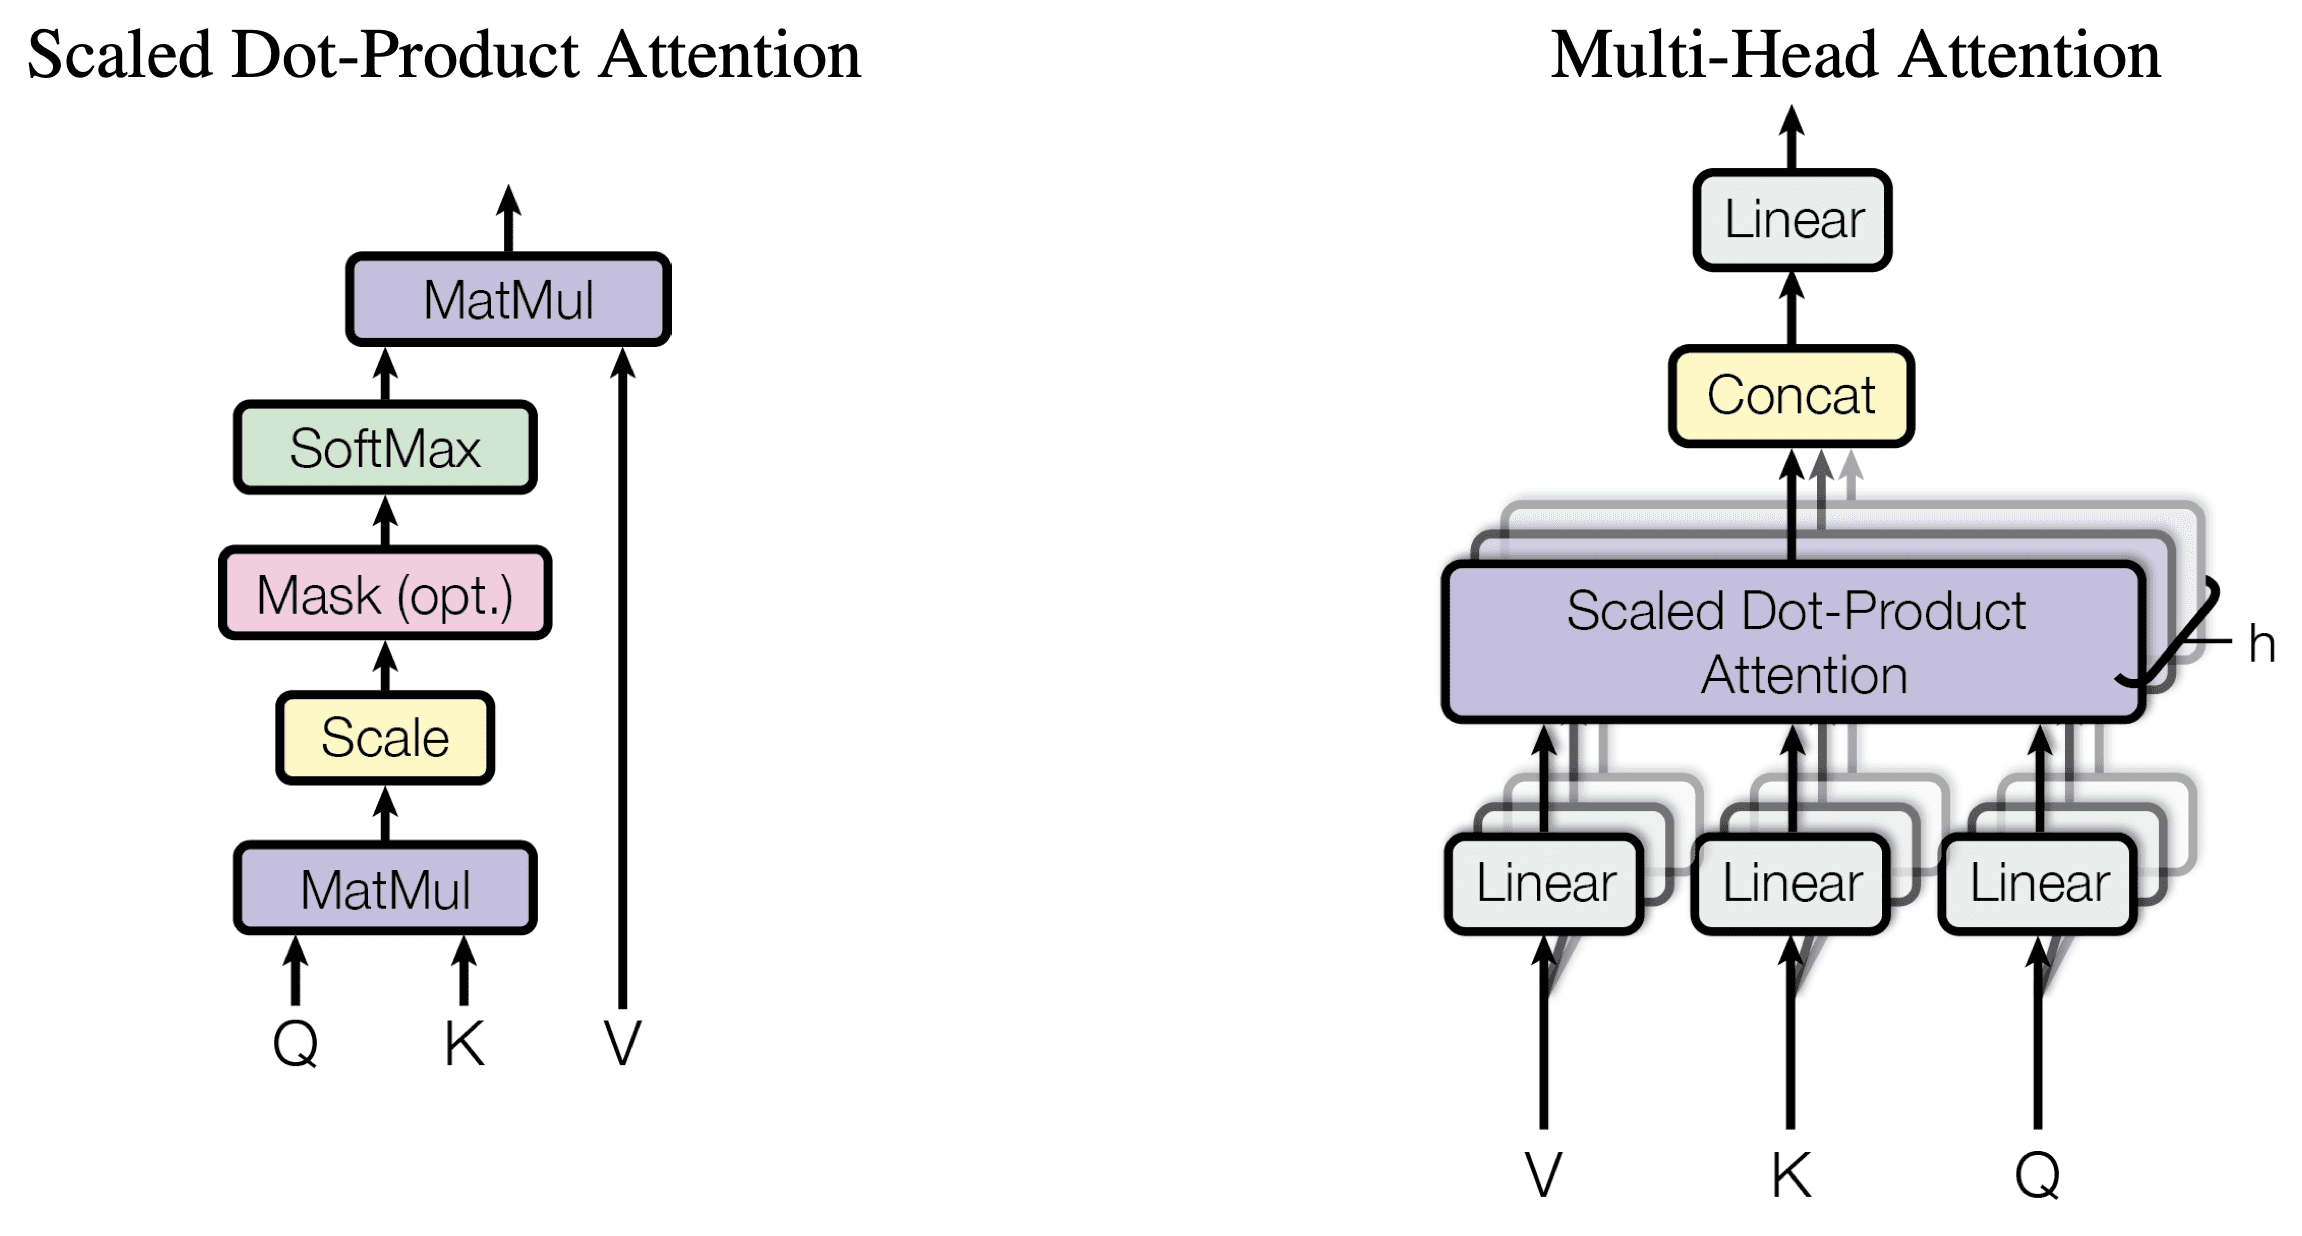
\includegraphics[height=6cm]{dotproduct_1.png}
    \label{fig:dotprod}
    \caption{On the left side, Scaled Dot-Product Attention. On the right side, Multi-Head Attention is depicted, which encompasses multiple attention layers operating concurrently.\cite{attention}}
\end{figure}

As a result, the model may calculate attention scores that reflect the significance or relevance of various points within a sequence. Both the Transformer's encoder-decoder attention mechanism and its self-attention mechanism use the attention function. Let's examine the attention function in greater detail:

\begin{enumerate}
    \item Input Vectors:
    \begin{enumerate}
      \item The three input vectors used by the attention function are : Queries (Q), keys (K), and values (V)
        \item For self-attention and encoder-decoder attention, respectively, these vectors are formed from the output or embeddings of the preceding layer.


    \end{enumerate}

    \item Linear Transformations:
    \begin{enumerate}
      \item The input vectors (Q, K, and V) are linearly transformed using learnt weight matrices before to generating attention ratings.
        \item With the aid of this transformation, the model is able to project the input vectors into a fresh space that more accurately depicts pertinent relationships.


    \end{enumerate}

    \item Dot Product Similarity:
    \begin{enumerate}
         \item The similarity between each key vector (K) and the query vector (Q) is calculated by the attention function using the dot product.
        \item The alignment or agreement of their orientations is measured by the dot product, which then records the similarity between the vectors.


    \end{enumerate}

    \item Scaling:
    \begin{enumerate}
       \item The dot product is adjusted by scaling it with the square root of the dimensionality of the key vectors to prevent big dot products from producing gradients with high magnitudes 
        \item The scaling helps to stabilize the training process and makes sure that the dot products are within a realistic range.


    \end{enumerate}

    \item Attention Scores and Softmax:
    \begin{enumerate}
         \item To determine attention scores, the scaled dot products are run through a softmax function.
        \item The scores are normalized using the softmax function to ensure that they add up to 1 and accurately reflect the relative weight or importance given to each position.


    \end{enumerate}

    \item Weighted Sum of Values:
    \begin{enumerate}
       \item The matching values (V) associated with the key vectors item are weighted using the attention ratings derived from the softmax function. 
      \item The attention function's ultimate result is produced by adding the weighted sum of the values.


    \end{enumerate}

    \item Multiple Attention Heads:
    \begin{enumerate}
        \item The model can pay attention to various patterns or dependencies inside the input sequence thanks to the attention function's many attention heads.
        \item Each attention head produces its own set of attention scores and output and has a unique set of learning weight matrices for linear transformations.


    \end{enumerate}
\end{enumerate}

By giving distinct places varied degrees of importance, the attention function allows the Transformer model to capture dependencies and relationships within a sequence. The Transformer can efficiently model long-range dependencies and produce contextually informed representations during both training and inference by incorporating self-attention and encoder-decoder attention methods.

% \subsubsection{Scaled Dot-Product Attention}

% The attention mechanism employed in our study is denoted as "Scaled Dot-Product Attention" (Figure \ref{fig:dotprod}). The input to this attention mechanism consists of queries, keys with a dimensionality of $d_k$, and values with a dimensionality of $d_v$. To calculate the weights assigned to the values, we perform dot products between the query and each key, scale them by a factor of $\sqrt{d_k}$, and then apply the softmax algorithm.

% In practice, the attention function is computed simultaneously for a set of queries that are organized into a matrix Q. Similarly, the keys and values are combined into matrices K and V, respectively. The output matrix is determined using the following calculation:

% \begin{center}
%     $
%     Attention(Q, K, V) = softmax(\frac{QK^T}{\sqrt{d_k}})V
%     $
% \end{center}

% Additive attention and dot-product (multiplicative) attention are the two most often employed attentional functions. The only difference between dot-product attention and our technique is the scaling factor, which is $\frac{1}{\sqrt{d_k}}$. The compatibility function is computed using additive attention, employing a feed-forward network with a single hidden layer. While both methods are theoretically equivalent in terms of complexity, in practice, dot-product attention proves to be faster and more space-efficient. This is due to its ability to leverage highly optimized matrix multiplication code for implementation.

% For bigger values of $d_k$, additive attention outperforms dot product attention without scaling, although the two processes perform comparably for small values of $d_k$. We postulate that as the dimensionality ($d_k$) of the query and key vectors increases, the magnitudes of the dot products also grow, thereby compelling the softmax function towards regions characterized by very small gradients\footnote{Consider the assumption that the components of $q$ and $k$ are independent random variables with a mean of 0 and a variance of 1. This assumption aids in illustrating the reason behind the magnification of dot products. Consequently, their dot product, $q \cdot k = \sum_{i=1}^{d_k} q_ik_i$, has an average value of 0 and a variance of $d_k$.}. To counterbalance this effect, we scale the dot products by $\frac{1}{\sqrt{d_k}}$.


% \subsubsection{Multi-Head Attention}

% We discovered that linearly projecting the queries, keys, and values with separate learned linear projections to dimensions $d_k$, $d_k$, and $d_v$ respectively, proved to be advantageous compared to employing a single attention function with $d_{model}$-dimensional keys, values, and queries. Consequently, the attention function is applied concurrently to each of the projected versions of queries, keys, and values, resulting in output values of dimension $d_v$. These output values are subsequently concatenated and projected once again, as illustrated in Figure \ref{fig:dotprod}.


% The utilization of multi-head attention in the model enables the simultaneous attention to be directed towards multiple representation subspaces at different positions. This capability allows for the joint consideration of diverse sets of data. In contrast, when employing a single attention head, the averaging process inhibits the model's ability to jointly attend to data across different representation subspaces and positions.

% \begin{center}

%     MultiHead($Q, K, V$) = Concat($head_1, ..., head_h$)$W^{O}$
    
%     where $head_i$ = Attention($QW_i^{Q}, KW_i^{K}, VW_i^{V}$)

% \end{center}

% The projections in this context refer to matrices $W_i^{Q} \in \mathbb{R}^{
% d_{model}×d_k}$, $W_i^{K} \in \mathbb{R}^{
% d_{model}×d_k}$, $W_i^{V} \in \mathbb{R}^{
% d_{model}×d_v}$.

% In this study, we employ a configuration consisting of $h$ = 8 parallel attention layers, commonly referred to as heads. For each attention head, we set the dimensions of the keys ($d_k$) and values ($d_v$) as $d_{model}/h$ = 64. This choice is made to ensure a comparable overall computing cost to that of single-head attention with the full dimensionality, despite the reduced dimensionality in each individual head.


% \subsection{Applications of Attention in a Transformer}

% \begin{itemize}
%     \item In "encoder-decoder attention" layers, memory keys and values are derived from the encoder's output, while queries are obtained from the preceding decoder layer. Consequently, the decoder can undertake the position in the input sequence.
%     \item The encoder incorporates self-attention layers. All of the keys, values, and queries in a self-attention layer are derived from the same source, in this instance the encoder's output from the layer below. Each position within the encoder has access to all positions in the stratum beneath it.
%    \item Similar to this, the self-attention layers of the decoder allow each position to pay attention to all positions preceding it. To preserve the decoder's auto-regressive property, we must prohibit leftward information flow. We implement this within scaled dot-product attention by masking (setting to) all input values of the softmax that correspond to unauthorized links.



 
% \end{itemize}

% \subsection{Why Self-attention}
%  We are going to compare various features of the self-attention layers to the recurrent and convolutional layers regularly utilized for mapping one variable-length sequence of symbol representations
% ($x_1, ..., x_n$) to another sequence of equal length ($z_1, ..., z_n$), with $x_i, z_i \in \mathbb{R}^d$, such as a hidden
% layer in a typical sequence transduction encoder or decoder. Motivating our usage of self-attention we
% can consider three desiderata.

% One is the aggregate computational complexity of every layer. The amount of computation ehich can be parallelized is set by the minimum number of sequential operations required.


% The third area of interest is the examination of long-distance dependencies within a network. Several sequence transduction activities are significantly hampered by the acquisition of long-range dependence. The distance that signals must travel in both forward and reverse directions has an impact on the network's ability to understand these dependencies. The learning of long-range dependencies is made easier by the short distances that these routes have between any two points in the input and output sequences. As a result, among networks made up of various layer types, a comparison of the maximum path length between any two points in the input and output sequences is made.

\section{BERT}

Google AI Language researchers recently published a paper titled "Bidirectional Encoder Representations from Transformers"(BERT \cite{BERT}). It resulted in heated conversations and debates in the machine learning field by revealing novel discoveries in a broad range of NLP tasks. These include Question Answering and Natural Language Inference among others.

BERT contributed significantly to language modelling by employing bidirectional training of the Transformer, a notable model employing attention mechanisms. Previous approaches differ from this one by processing text sequences in a left-to-right order or by combining left-to-right and right-to-left orientations in training. Initial findings indicate that a language model trained in two orientations has a greater understanding of linguistic context and flow than its counterparts trained in a single direction. The researchers introduce the Masked Language Model (MLM), a ground-breaking strategy that pioneers bidirectional training in models where such an approach was previously impractical.





\subsection{Background}

Transfer learning in computer vision entails preparatory training of a neural network model on a well-known task, and refining it afterwards to serve as the base to be constructed for a new model with a specific purpose. Recent research has shown that a kindred approach can be useful for a wide array of natural language tasks.

A distinct approach is feature-based training, prevalent in NLP applications and illustrated in the most recent ELMo publication. A pre-trained neural network is used to generate word embeddings, subsequently utilized as features in NLP models.



\subsection{Explaining BERT}

BERT is a sophisticated language model designed to enhance the complexity of machine learning and the understanding of linguistic context. It was initially developed by Google and has since evolved into a potent NLP tool.

BERT's foundation is the Transformer architecture and functions as a mechanism that can comprehend contextualized relationships related to words and their subcategories in various situations and contexts. A typical Transformer is comprised of a decoder that produces a prediction and an encoder that scans the input text. However, BERT only employs the encoder mechanism, which is consistent with its objective of developing a language model.


In contrast to standard models, which read text word by word, the Transformer encoder utilized by BERT scans the whole sequence of terms simultaneously. This allows it to comprehend a word's contextual behaviour in regard to the entirety of its surroundings, effectively rendering it bidirectional. However, nondirectional would be a better term because it does not inherently favour any particular direction.
A series of tokens (words or subwords) are implanted into vectors by the Transformer encoder prior to neural network processing. The product consists of a series of H-dimensional vectors, each correlated with a token with the same index as the input.

It is challenging to determine a forecasted objective at the time of language model training. Numerous models forecast the following term in a sequence. However, this strategy restricts context-based learning opportunities. BERT employs two distinct training techniques to surmount this challenge.

\begin{figure}[!h]
    \centering
    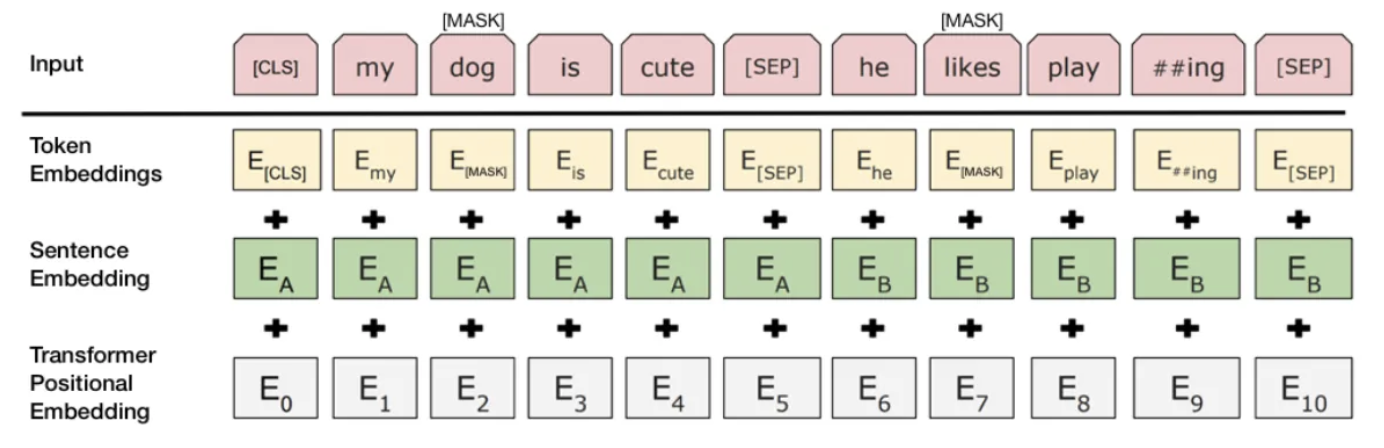
\includegraphics[width=0.7\textwidth]{images/nsp.png}
    \label{fig:nsp}
    \caption{Input representation for BERT\cite{BERT}}
\end{figure}


The first of these techniques involves the pre-training of deep bidirectional depictions of unassigned wording. This is accomplished through the use of joint conditioning on the left and right contexts across all layers. Consequently, state-of-the-art models for a variety of tasks can be created by incorporating a single output layer into the preliminary trained BERT model. These activities, such as language inference and query answering, do not necessitate significant architectural modifications.

BERT uses masked language modelling as a strategy to enhance instruction. In this method, a portion of the input tokens are unsystematically muted, and the model is then instructed to determine the original vocabulary id of the muted word depending on the circumstances. This technique authorizes the model to understand not only the connotation of the words but also their relationships within a phrase.

\begin{figure}[!h]
    \centering
    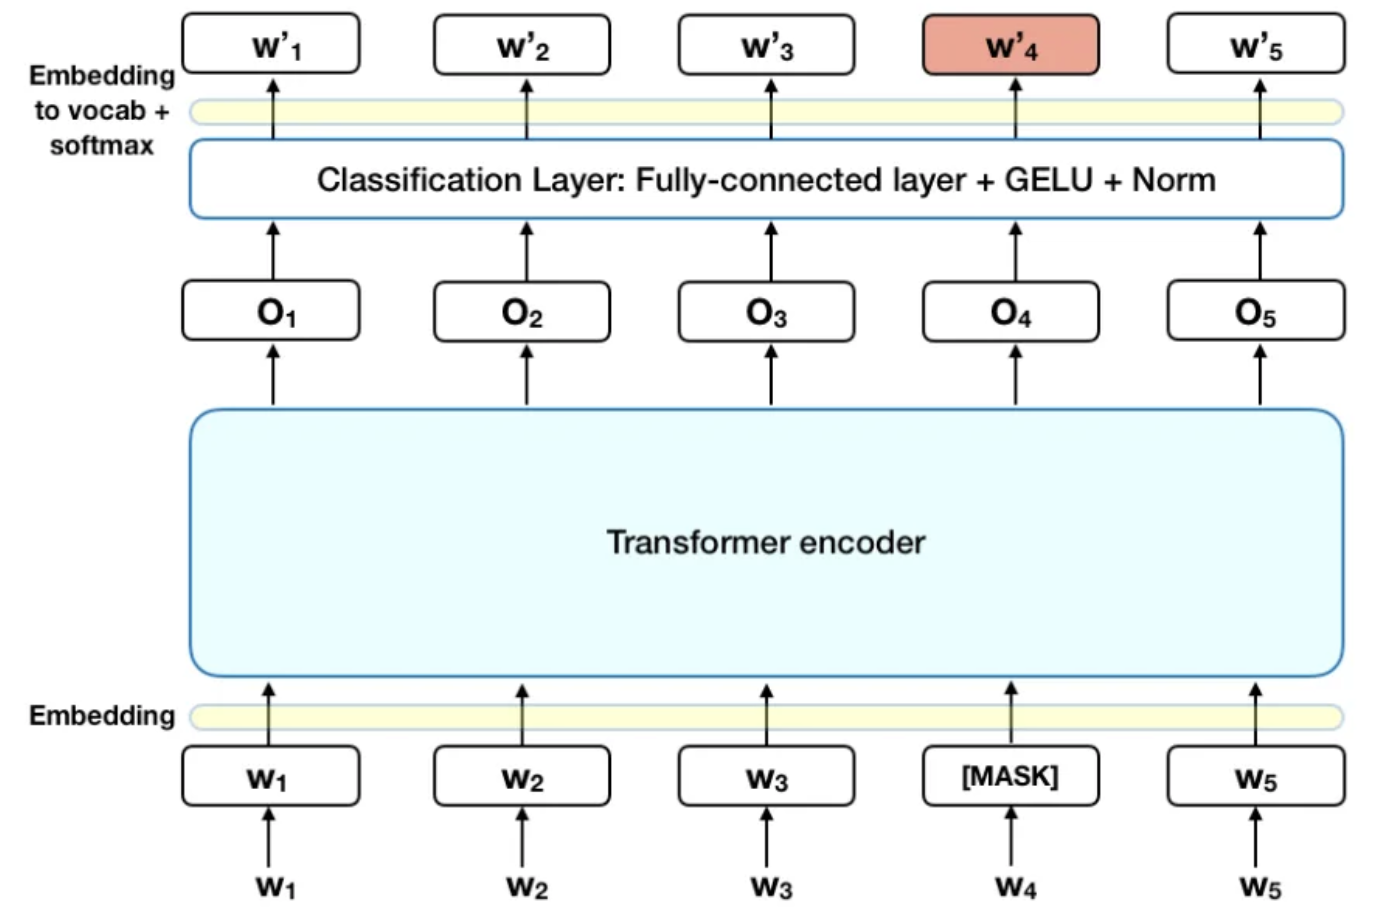
\includegraphics[width=0.7\textwidth]{images/mlm.png}
    \label{fig:mlm}
    \caption{BERT functioning mechanism breakdown\cite{towardsdatascience}}
\end{figure}



Due to its context-centred approach and non-directional nature, BERT provides a reliable method for language modelling. It is a powerful tool in the disciplines of AI and machine learning due to its pre-training and fine-tuning procedures, which allow it to execute exceptionally well on diverse NLP jobs. It has proven to be both theoretically simple and practically effective, allowing for further language processing research and development.

The diagram depicts the operational workflow of the Transformer encoder. As system inputs, a collection of tokens initially transformed into vector embeddings serve. The neural network is then applied to these embedded vectors for processing. The final output of the system is a collection of H-dimensional vectors. Each output vector corresponds to an input token with the same index, and the output vectors are aligned with the input tokens.



In the field of language model training, defining a prediction objective is extremely complex. In numerous models, the method of predicting the next word in a series has been incorporated. However, this unidirectional method inherently restricts context-based learning. BERT employs two distinct training methods to mitigate the effects of these restrictions.





% \subsubsection{Masked LM (MLM)}

% Before feeding word sequences into the BERT, 15\% of each sequence's words are modified with a [MASK] token. Using the context provided by the non-masked words in the sequence, the model then attempts to predict the original value of the masked words. Technically, the output word prediction necessitates:





% \begin{itemize}
%      \item On top of the encoder output, a classification layer is added, and the output vectors are multiplied by the embedding matrix to generate the vocabulary dimension.
%      \item Determine the probability of each word in the lexicon using softmax.




% \end{itemize}

% \begin{figure}[!h]
%     \centering
%     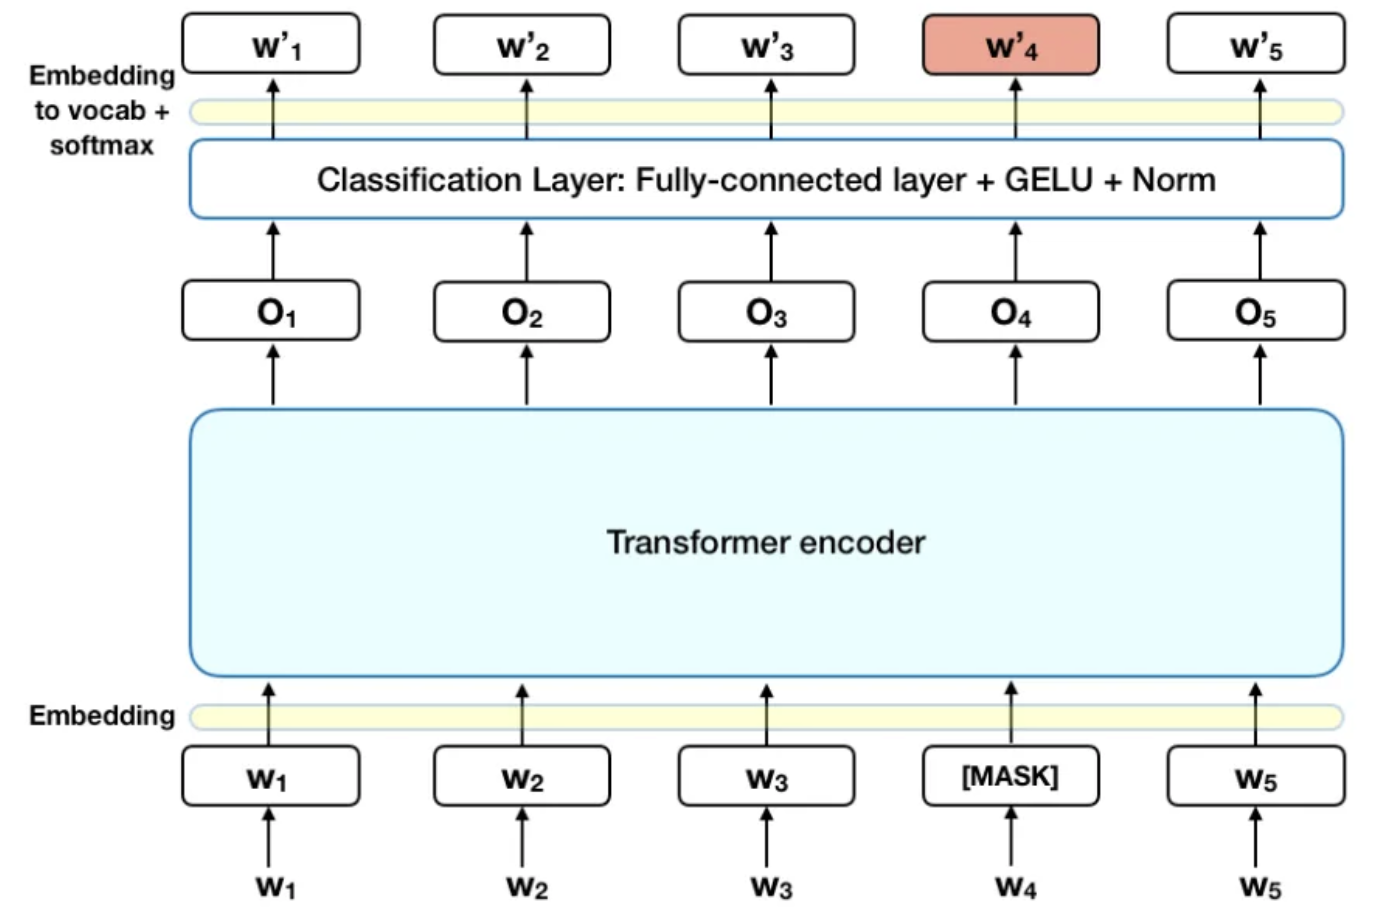
\includegraphics[width=0.7\textwidth]{images/mlm.png}
%     \label{fig:mlm}
%     \caption{NLP State-of-the-art language model}
% \end{figure}

% The BERT loss function disregards the prediction of non-masked terms and only considers the prediction of masked values. Compared to directional models, the model's delayed convergence rate is compensated for by its enhanced context awareness.



% \subsubsection{Next Sentence Prediction (NSP)}

% As the Bidirectional Encoder Representations from Transformers (BERT) model is being trained, it is supplied pairs of sentences. The primary objective is to equip the model with the ability to determine whether the second sentence of a pair follows the first in the original text. Half of the examples in the training process consist of pairings in which the second sentence follows the first in the original context, while the other half consist of pairs in which the second sentence is randomly selected from the corpus. It is anticipated that the sentence selected at random will lack cohesion with the previous sentence. During the training phase, the input is processed prior to being fed to the model so that it can distinguish between the two sentences that comprise the combination.







% \begin{itemize}
%     \item The first sentence begins with a [CLS] token, and each subsequent sentence ends with a [SEP] token.
%     \item Each token contains an embedded sentence that identifies either Sentence A or Sentence B. Sentence embeddings and token embeddings with a vocabulary of 2 share a similar concept.
%     \item Each token is assigned a positional embedding to indicate its position within the sequence. This paper describes the theory and practice of positional embedding.

% \end{itemize}


% \begin{figure}[!h]
%     \centering
%     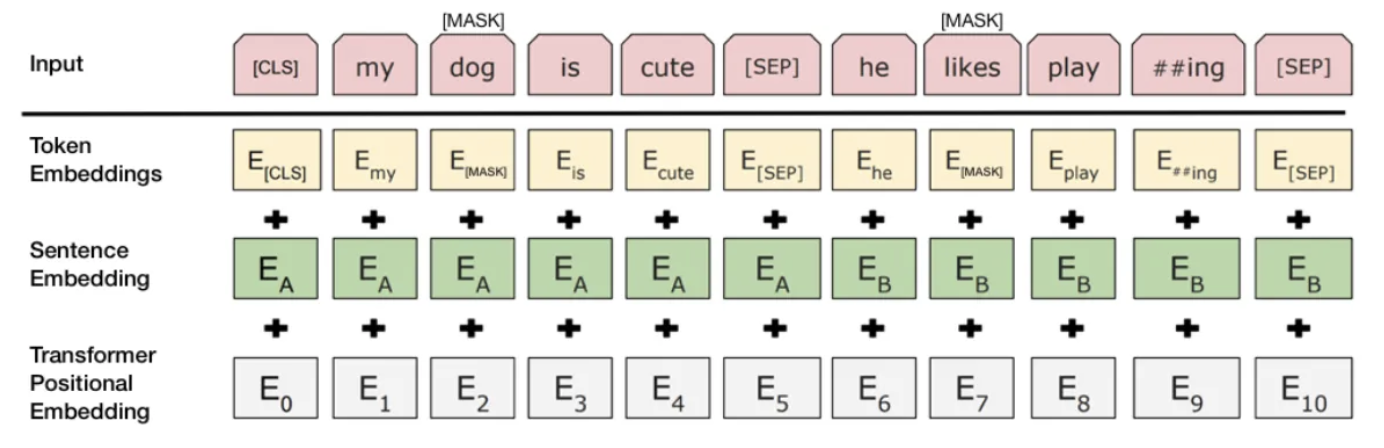
\includegraphics[width=0.7\textwidth]{images/nsp.png}
%     \label{fig:nsp}
%     \caption{Input representation for BERT}
% \end{figure}

% The following steps are performed to determine whether the second statement is in fact related to the first.




% \begin{itemize}
%     \item The entire input sequence goes through the Transformer model.
%     \item The output of the [CLS] token is altered into a 2×1 shaped vector, with the help of a simple classification layer (learned matrices of weights and biases).
%     \item The usage of softmax in order to calculate the likelihood of IsNexSequence.
% \end{itemize}

% When training the BERT model, Masked LM and Next Sentence Prediction are simultaneously learnt in order to minimize the merged loss function of our two techniques.


\subsection{Usage of BERT (Fine-tuning)}

The BERT paradigm can be easily applied to certain jobs and does not necessitate significant changes to the fundamental model. Fine-tuning is a technique that can be put into application to a variety of linguistic tasks with little modification to the fundamental model.

A classification layer is added to the Transformer yield for the [CLS] token for classification tasks like sentiment analysis, simulating the Next Sentence classification process. Due to its aptitude for comprehending context and semantic relationships, BERT is now able to solve text categorization problems using a similar architecture.


When it comes to Question Answering Tasks, BERT is tasked with finding the answer inside a given written succession after being given a question in regards to it. The model is effectively instructed to perform Question Answering tasks by teaching it two additional vectors that specify the beginning and conclusion of the answer.

For NER, BERT is given a text sequence and instructed to identify different kinds of entities (such as Person, Organization, Date, etc.) that are contained in the written work. The model is able to correctly detect and categorize various items within the text because it has been instructed by feeding the output vector of every token to a layer used for classification purposes that forecasts the labelling of NER.



Between the initial BERT practice and the fine-tuning procedure, the majority of hyper-parameters remain stable. The original BERT publication, however, offers detailed instructions on the hyper-parameters which might necessitate adjusting throughout this procedure. The BERT team has been successful in obtaining cutting-edge results using these fine-tuning methods on a wide spectrum of difficult natural language tasks.

% \subsection{Takeaways}

% Even at very large sizes, a model's size has a major impact on how well it performs. The comparison of BERT\_large and BERT\_base makes this idea very evident. The more comprehensive model of its kind is the former, which has 345 million parameters. In tasks carried out on a smaller scale, empirical evidence has demonstrated a definite advantage over the BERT basic model. The latter has the same architecture but has 110 million fewer parameters than the former.


% Given enough training data, the connection between the number of training steps and model accuracy shows that increasing the number of training steps often results in an increase in model accuracy. This fact is particularly clear in the MNLI problem, where training the BERT\_base model with 1 million steps (with a batch size of 128,000 words) results in a 1.0 \% gain in accuracy compared to training it with 500,000 steps while maintaining the batch size constant.

% Due to the fact that only 15\% of words are predicted in each batch, the Masked Language Model (MLM), the bidirectional training method used by BERT, converges more slowly than traditional left-to-right methods. After a limited number of pre-training stages, the bidirectional training methodology still outperforms left-to-right training despite its slower convergence. These details emphasize how creative BERT's method for handling jobs involving natural language processing is.

% \begin{figure}[!h]
%     \centering
%     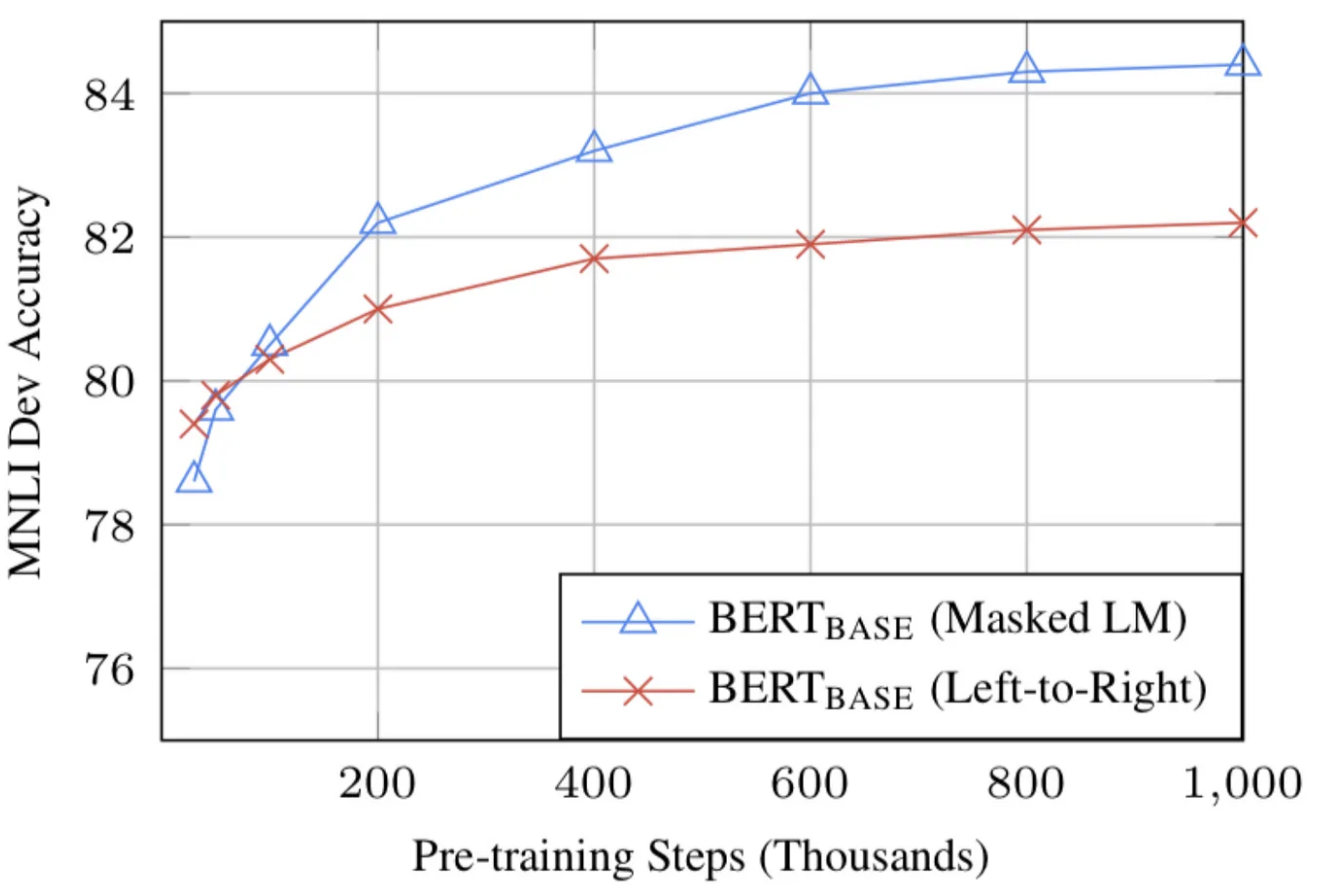
\includegraphics[width=0.7\textwidth]{images/takeaways.png}
%     \label{fig:takeaways}
%     \caption{My caption}
% \end{figure}

\section{Hugging Face}

Hugging Face\footnote{https://huggingface.co/} is primarily an open-source platform and library created exclusively for NLP jobs. Its goal is to democratize AI by giving academics and developers easy-to-use tools. Hugging Face has developed a thriving and welcoming community that encourages cooperation and knowledge exchange among NLP fans throughout the world.

\subsection{Features and Benefits}
Hugging Face is a valuable tool for NLP practitioners thanks to its many features and advantages. The enormous selection of pre-trained models, which includes the highly regarded BERT model, is one of its standout features. Hugging Face's Model Hub makes these models easily accessible, allowing transfer learning and hastening the creation of NLP applications.



The transformers library from Hugging Face also acts as a complete toolkit for creating, honing, and deploying NLP models. With a large number of utilities and abstractions available to developers, this library streamlines the entire model development life cycle. Pipelines, which are high-level APIs for typical NLP tasks like written content categorization and named entity recallection, are also included in the library, making it simple to create complex NLP systems.

Additionally, Hugging Face emphasizes teamwork and model sharing heavily. Its user-friendly platform allows academics and developers to share their models, building an ecosystem that is driven by the community and advantageous to all parties. The advancement of NLP is made possible by this collaborative atmosphere, which encourages the sharing of ideas, best practices, and novel strategies.



\subsection{Hugging Face's Integration of BERT}

Hugging Face was essential in getting BERT well-known and available to the NLP community. Hugging Face offers pre-trained BERT models through its Model Hub, allowing developers and researchers to take advantage of BERT's capability without the requirement for time-consuming training. Hugging Face's transformers library also provides seamless connection with BERT, enabling users to quickly and easily modify the model for particular NLP needs.


\chapter{Applying BERT for Translationese Classification}

\section{Model description}

The Bidirectional Encoder Representations from Transformers (BERT) pre-trained transformer model is fed data and modelled on a large body of English language data. It functions autonomously, indicating that it was trained on unlabeled, unprocessed material. The automated procedure utilized to give inputs and labels from these written documents enables the use of a vast quantity of publicly available data.




The BERT pre-training routine serves two distinct purposes. Beginning with masked language modelling (MLM), 15\% of the words in a sentence are randomly masked. The model is then applied to the entire concealed text to predict the hidden words. This approach does not employ recurrent neural networks (RNNs), which typically process words sequentially and autoregressive models such as GPT, which inherently mask future tokens. The MLM enables the model to learn a bidirectional representation of the text, in contrast to the unidirectional approach of other models.




BERT utilizes the next sentence prediction (NSP) objective during pre-training. In this instance, the model is provided with two masked sentences, which may or may not be consecutive sentences from the original text. The model is responsible for determining whether the second phrase follows promptly after the first.


During this pre-training phase, BERT creates its own interpretation and understanding language model of English from which it can extract features useful for a variety of subsequent tasks. If a set of labelled phrase data is provided, for instance, a conventional classifier is capable of being trained using the BERT model's generated features as inputs.




\section{Layers description}

\subsection{Linear}

The PyTorch linear layer is essential for linear transformations in deep learning models. It represents a layer that conducts a linear operation on the input data and is sometimes referred to as dense layer or linear transformation.

When creating a torch instance, the input and output sizes of the layer must be specified.nn.Linear. The number of input features is determined by the input size, whereas the number of output features is determined by the output size. Using a matrix multiplication and an optional bias term, this layer transforms the input data from the input size to the output size.


This linear layer is internally initialized with a bias vector and a weight matrix. By default, the biases are initialized to zero, and the weights are randomly selected from a uniform distribution.


\subsection{MaxPool1d}

The torchbearer, nn.MaxPool1d is a pooling operation that downsamples a one-dimensional input tensor in PyTorch. This technique is frequently used by convolutional neural networks (CNNs) to reduce the number of parameters and capture the most essential information by compressing the spatial dimensions of the input.



The kernel size and stride must be specified when establishing an instance of \\ Torch.nn.MaxPool1d. The stride specifies the size of the step between successive pooling operations, while the kernel size provides the size of the pooling window that glides across the input tensor. The maximum value of each pooling window is absorbed by the layer, and the remaining values are discarded.


The output value can be calculated as:

\begin{equation}
    out(N_i, C_j, k) = \max_{m=0,...,kernel\_size-1} input(N_i, C_j, stride * k + m)
\end{equation}


\subsection{Dropout1d}

The torchbearer, nn.Dropout1d layer regularization in PyTorch is used to prevent overfitting in deep learning models, particularly in sequential data processing tasks. During training, some input tensor components are set to zero at random with a specified probability, effectively "dropping out" some values. Using samples from a Bernoulli distribution, each forward call will, with probability p, result in the independent zeroing out of each channel.



When constructing a torch instance, it is necessary to specify the dropout probability, which determines the likelihood that an element will be set to zero during training. Each element of the input tensor is individually and element-by-element subjected to the dropout operation of the layer.




During training, the elements of the input tensor are randomly set to zero with the specified dropout probability by the Dropout1d layer. By avoiding an overreliance on particular traits, this helps the network to develop representations that are more robust and universal. During inference or evaluation, the layer scales the output by $\frac{1}{1-dropout\_prob}$ to ensure consistent output statistics.

\subsection{ReLU}

In PyTorch, the ReLU layer represents the torch.nn.ReLU (Rectified Linear Unit) activation function, a popular nonlinear activation function in deep learning models. As it operates element-by-element on the input tensor, ReLU nullifies negative values while keeping positive ones.


\begin{equation}
    ReLU(x) = {(x)}^{+} = \max(0, x)
\end{equation}

While building a torch, no extra parameters are required to be specified.instance of nn.ReLU. The ReLU activation function in the layer is simply applied to the input tensor.

In deep learning models, ReLU is a popular activation function due to its efficiency and simplicity. By adding non-linearity, the network, the model is able to learn complex representations and take in more expressive inputs. ReLU further reduces the problem of disappearing gradients because it does not saturate for positive values.

In conclusion, ReLU function activates the input tensor.

\subsection{Tanh}

The torch.nn.Tanh function in PyTorch represents the hyperbolic tangent activation function, a non-linear activation function often used in deep learning models. The torch.nn.Tanh function performs an element-by-element action on the input tensor, converting each element to its corresponding hyperbolic tangent value.

Each component of an input tensor, x, is transformed by the torch.nn.Tanh function into its corresponding hyperbolic tangent value, $tanh(x)$. When it reaches saturation, the hyperbolic tangent function returns values between -1 and 1. Mathematically speaking, it is:


\begin{equation}
    Tanh(x) = tanh(x) = \frac{exp(x) - exp(-x)}{exp(x) + exp(-x)}
\end{equation}

The hyperbolic tangent function torch.nn.Tanh, a non-linear function, is used to incorporate non-linearity into the network, enabling the model to learn complex representations and capture more expressive features. Similar to the sigmoid function, it squashes the input values; however, it is zero-centered and has a greater slope towards zero. This can help with the fading gradient problem and increase its applicability for particular professions.

In conclusion, the torch.nn.tanh function applies the hyperbolic tangent activation function element-by-element to each element in an input tensor to determine the associated hyperbolic tangent value. Deep learning models typically employ this non-linear activation function.


\subsection{RReLU}

The RReLU (Randomized Leaky Rectified Linear Unit) layer is an activation function in PyTorch that augments the standard Leaky ReLU function with randomness during training. Each member of the input tensor receives a random leaky ReLU transformation from RReLU, with a different random slope within a predetermined range. When drawing conclusions, it behaves like a standard ReLU.

When building an instance of torch, the lower and upper bounds for the possible range of random slopes can be optionally supplied.nn.RReLU. If nothing else is supplied, the default range is between 0.125 and 0.3333333333333333.


\begin{equation}
RReLU(x) =\begin{cases} 
          x & x\geq 0 \\
          ax & otherwise\\
       \end{cases}
\end{equation}

During training by the torch, each input tensor element is given a distinct random slope within the predefined range. As a result, the activations are given some stochasticity, which can work as a regularizer and help prevent overfitting. During inference or evaluation, the layer behaves like a standard ReLU, setting negative values to zero and keeping positive values.

The torch.nn.RReLU layer can be used as a drop-in replacement for other activation functions, such as ReLU, in deep learning models. Controlled unpredictability is a benefit that can be added during training to improve model performance and generalization.

In conclusion, by applying a randomized leaky ReLU activation function to an input tensor during training, the torch.nn.RReLU layer introduces randomization and acts as a regularizer. During inferencing, it functions as a conventional ReLU activation function.



\section{Model variations}

The BERT model was initially offered in two configurations: "base" and "large." It supports both case-sensitive and case-insensitive text inputs. By deleting accent markers in uncased versions, the model is made simpler. In order to support Chinese and other languages, cased and uncased variants of the model were eventually made accessible. Following that, whole-word masking took the place of the previous sub-piece masking strategy, indicating a change in preprocessing methods. This switch was also announced together with the debut of two new models. The introduction of 24 tiny BERT models, primarily designed for scenarios with computing constraints, was then made after these.

Translationese has been detected using the bert-base-uncased model.

\begin{center}
    
\begin{tabular}{ |p{8cm}||p{3cm}|p{3cm}|  }
 \hline
Model	&\#params	&Language\\
 \hline
bert-base-uncased	&110M	&English\\
bert-large-uncased	&340M	&English\\
bert-base-cased	&110M	&English\\
bert-large-cased	&340M	&English\\
bert-base-chinese	&110M	&Chinese\\
bert-base-multilingual-cased	&110M	&Multiple\\
bert-large-uncased-whole-word-masking	&340M	&English\\
bert-large-cased-whole-word-masking	&340M	&English\\
 \hline
\end{tabular}
\captionof{table}{BERT variations\cite{hug}}

\end{center}

\chapter{Experimental Study}

\section{Data}

\subsection{Explaining the data}

The dataset used in this thesis is the \quotedblbase{}Corpus of English Translated Texts and Originals (CETTO)’’ (Doherty et al., 2021), available on Zenodo: \href{https://zenodo.org/record/5596238}{zenodo.org/record/5596238}. 
Out of the single-source monolingual data sets, only mono\_de\_en and mono\_es\_en were used.
This data was split into 2 sections: DE-EN and ES-EN.
Each data set consists of 42.260 English texts, of which 21.130 translated texts and 21.130 non-translated texts.

Both translated and original texts are taken from diverse genres, such as fiction, non-fiction, news articles, and technical documents, to ensure a representative sample of English texts and specific vocabulary. 

\subsection{Preprocessing Procedure}

Before implementing the classification models, the data set needs to be processed in advance to ensure the optimal performance of both feature engineering and feature learning approaches. The pre-processing steps were done with a pre-trained tokenizer \cite{huggingfaces}. 

Import tokenizer :
\begin{lstlisting}[language=Python]
    tokenizer = BertTokenizer.from_pretrained(name)
\end{lstlisting}

The lowercase texts undergo tokenization with the usage of WordPiece and a 30,000-sized vocabulary. Subsequently, the model's inputs are structured in the following manner:

\begin{center}
    [CLS] First Sentence [SEP] Second Sentence [SEP]
\end{center}

There exists a 50\% probability that the First Sentence and Second Sentence are sequential sentences in the original body of text, the corpus. In other scenarios, the chosen sentence might be a random selection from the corpus. Here, a sentence is defined as a contiguous span of text, generally exceeding a single sentence in length. The sole requirement for these "sentences" is that their combined length should not surpass 512 tokens.

It is crucial to note that the term "sentence" as utilized here, does not strictly refer to a single sentence in traditional syntactic terms, but rather to a continuous stretch of text which might be lengthier than a conventional phrase. Only one condition is a prerequisite, namely the fact that the combined size of two ”sentences” must not be over 512 tokens.

The outlined specifications for the masking procedure for each sentence are as follows:

\begin{itemize}
    \item Fifteen percent (15\%) of the tokens within a sentence are subjected to masking.
    \item Among the masked tokens, eighty percent (80\%) are substituted with the [MASK] token.
    \item The masked tokens are switched with randomly selected tokens that are not the same as the original ones in 10\% of the cases
    \item The remaining ten percent (10\%) of the masked tokens remain unchanged.
\end{itemize}

Extract input\_ids, attention\_masks and token\_type\_ids:

\begin{lstlisting}[language=Python]
    for text in X:
        out_dict = tokenizer.encode_plus(
            text,                  # Text for encoding
            truncation = True,
            max_length = max_len,
            add_special_tokens = True, # Adding '[SEP]', '[CLS]'
            padding = 'max_length',
            return_tensors = 'pt',     # This line returns a tensor.
            return_attention_mask = True,
            return_token_type_ids=True,
        )
\end{lstlisting}

After this operation, we construct a DataLoader with TensorDataset(input\_ids, attention\_masks, token\_type\_ids, labels), batch\_size and shuffle (boolean value).


\section{Results}

In the process of obtaining the best accuracy, I initially passed all the texts through the BERT model which was set in test mode, that is, backward() was not done through the network. The [CLS] output for a text was a tensor with a size of 768. Then I trained several Neural Networks (NN) to see which ones presented the best accuracy. The best models from Experiment 1 were used further, in Experiment 2.

\subsection{Experiment 1}

Experiment 1 consisted of finding the best model for fine-tuning. The tested models exhibited variations in both the type and quantity of layers employed, as well as various activation functions. The number of epochs was the same for all, this being 50. The learning rate took values from the following array 
$[4*10^{-5}, 4*10^{-4}, 2*10^{-4}, 10^{-4},$ \newline $6*10^{-3}, 4*10^{-3}, 2*10^{-3}, 10^{-3}]$. The batch size remained constant at 32.

\subsubsection{Model 1}

% Model arhitecture :
% \begin{lstlisting}[language=Python]
%     class MLP(nn.Module):
%       def __init__(self):
%         super().__init__()
%         self.layer1 = nn.Linear(768, 256)
%         self.layer2 = nn.Linear(256, 2)
%         self.activation = nn.ReLU()
%       def forward(self, x):
%         out = self.activation(self.layer1(x))
%         out = self.layer2(out)
%         return out
% \end{lstlisting}

Model 1 is a multi-layer perceptron (MLP) implemented using PyTorch's nn.Module class.

The Multilayer Perceptron (MLP) architecture encompasses hidden layers and an output layer. The model is expected to have a size of 768, which suggests that it is designed to work with inputs of length 768.

In the initialization method (\_\_init\_\_), the model's architecture is defined. It consists of two linear layers (self.layer1 and self.layer2) with 256 and 2 units, respectively. The nn.Linear class corresponds to a fully connected layer, wherein each neuron establishes connections with every neuron present in the preceding layer. The initial linear layer receives an input tensor with a dimensionality of 768 and generates an output tensor with a dimensionality of 256. Subsequently, the succeeding linear layer accepts the output from the preceding layer (256) and produces a tensor with a dimensionality of 2. This configuration indicates that the model is specifically tailored for a binary classification task.

The function nn.ReLU() is employed as the initiation procedure within a Multi-Layer Perceptron (MLP) architecture, situated between two linear layers. The Rectified Linear Unit (ReLU) serves as a widely utilized activation function, introducing non-linearity into the model, thus facilitating the learning of intricate patterns within the data.

The forward method delineates the forward pass of the model. It accepts the input 'x' and guides it through the various layers of the model. The process commences with the input being passed through the initial linear layer, denoted as 'self.layer1'. Subsequently, the ReLU activation function is applied to this input, denoted as 'self.activation', performing element-wise activation. The resultant tensor is thereafter passed through the second linear layer, denoted as 'self.layer2', to generate the final output. This output stands for the predicted class probabilities pertinent to the binary classification task.

Conclusively, the above-described model architecture is a basic MLP comprising two hidden layers, using ReLU activation in between the layers, and a terminal linear layer designed for classification.







\begin{center}
    \begin{figure}[!h]
        \centering
        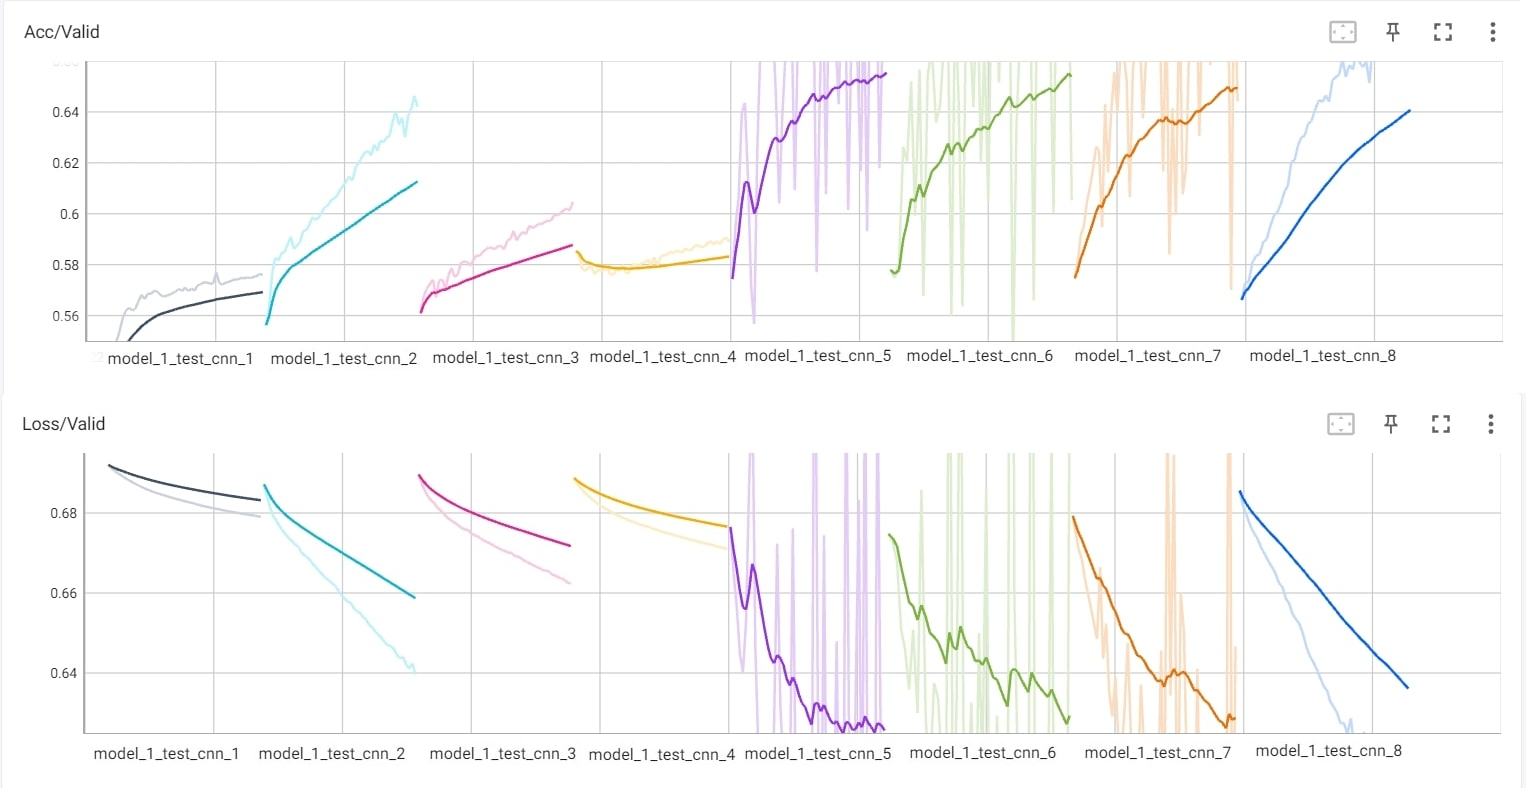
\includegraphics[width=\textwidth]{images/exp1_acc1+loss1.jpg}
        \label{fig:exp1_model1}
        \caption{Results for Model 1 at different learning rates}
    \end{figure}
\end{center}



\subsubsection{Model 2}

% Model arhitecture :
% \begin{lstlisting}[language=Python]
%     class MLP(nn.Module):
%       def __init__(self):
%         super().__init__()
%         self.layer1 = nn.Linear(768, 256)
%         self.layer2 = nn.Linear(256, 2)
%         self.activation = nn.ReLU()
%         self.drop = nn.Dropout1d(p=0.1)
%       def forward(self, x):
%         out = self.activation(self.layer1(x))
%         out = self.drop(out)
%         out = self.layer2(out)
%         return out
% \end{lstlisting}

Model 2 is also a multi-layer perceptron (MLP) with dropout regularization implemented using PyTorch's nn.Module class.

The MLP is similar to the previous model. The input to the model is expected to have a size of 768.

In addition to the previous model, this model also includes a dropout layer (self.drop) with a probability $p=0.1$. This particular layer randomly sets to 0 a fraction of input units uring training, this particular layer sets arbitrarily to 0 a portion of input units, thereby preventing overfitting by diminishing the dependence on specific neurons.


% In addition to the layers and activation function, this model also includes a dropout layer (self.drop). Dropout is a regularization technique that randomly sets a fraction of input units to 0 during training, which helps prevent overfitting by reducing the reliance on specific neurons.

% In the initialization method (\_\_init\_\_), the architecture is defined with the same linear layers as before, and the ReLU activation function is applied between the layers. Additionally, a dropout layer with a dropout rate of 0.1 is added.

% In the forward method, the input x is passed through the layers of the model. After the first linear layer and activation function, the output is passed through the dropout layer (self.drop) before proceeding to the second linear layer. The dropout layer randomly sets a fraction of the activations to 0, promoting the model's robustness by reducing over-dependence on specific activations.

% The final output of the model represents the predicted class probabilities for a binary classification task, as in the previous model.

In summary, this model extends the previous MLP by incorporating dropout regularization.

\begin{center}
    \begin{figure}[!ht]
        \centering
        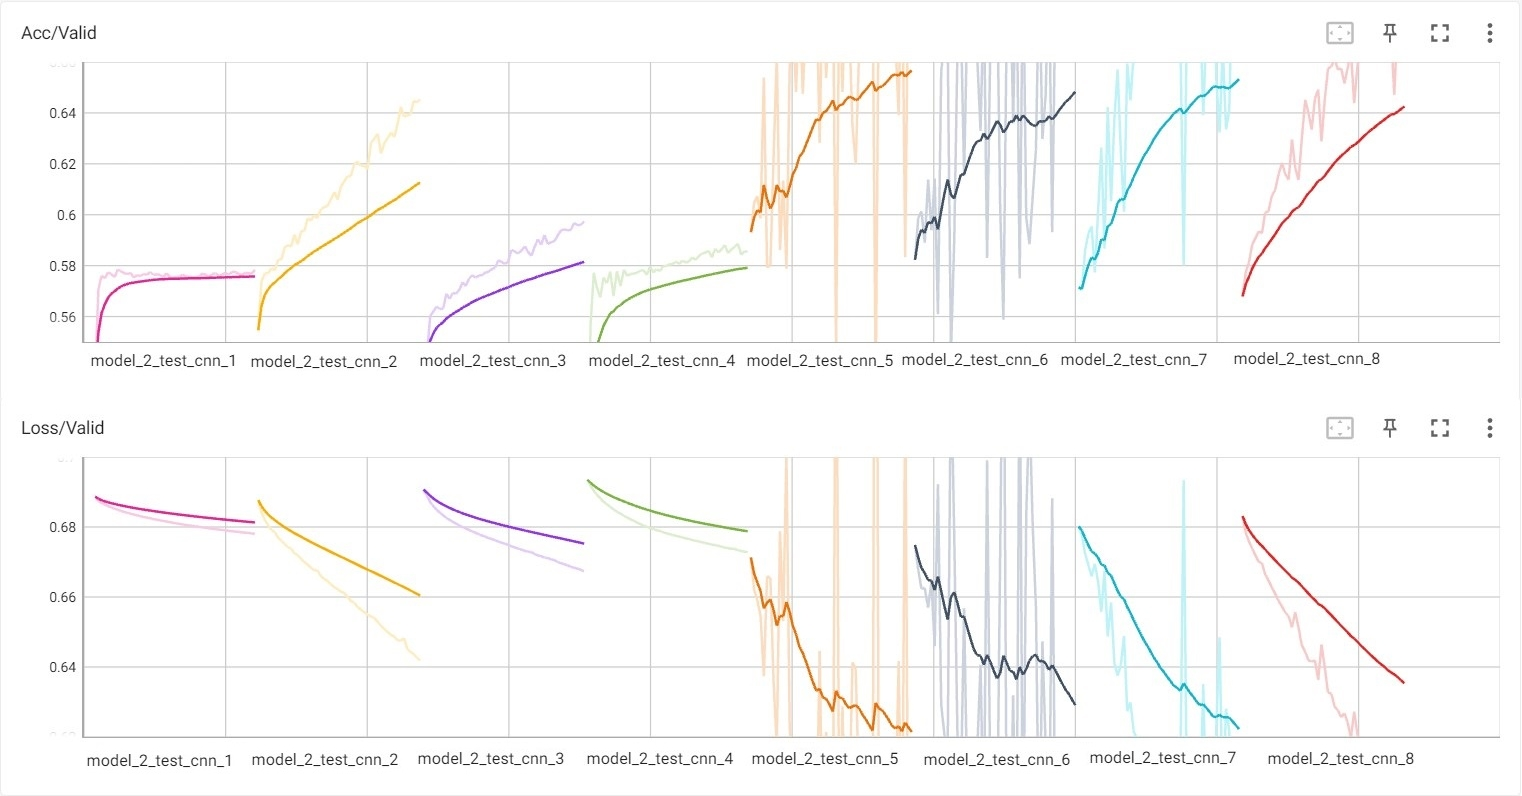
\includegraphics[width=\textwidth]{images/exp1_acc2+loss2.jpg}
        \label{fig:exp1_model2}
        \caption{Results for Model 2 at different learning rates}
    \end{figure}
\end{center}


\subsubsection{Model 3}

% Model arhitecture :
% \begin{lstlisting}[language=Python]
%     class MLP(nn.Module):
%       def __init__(self):
%         super().__init__()
%         self.layer1 = nn.Linear(768, 256)
%         self.layer2 = nn.Linear(256, 2)
%         self.activation = nn.Tanh()
%         self.drop = nn.Dropout1d(p=0.1)
%       def forward(self, x):
%         out = self.activation(self.layer1(x))
%         out = self.drop(out)
%         out = self.layer2(out)
%         return out
% \end{lstlisting}

Model 3 is a multi-layer perceptron (MLP) with dropout regularization and a hyperbolic tangent activation function implemented using PyTorch's nn.Module class. Tanh is an activation function used on each layer 1 output. This can be observed in the following chart:

% However, instead of using the ReLU activation function, this model utilizes the hyperbolic tangent (Tanh) activation function (self.activation). The Tanh activation function maps the input values to the range [-1, 1], allowing for non-linear transformations.

% Similar to the previous models, this MLP has two hidden layers and one output layer. The input to the model is expected to have a size of 768.

% In the initialization method (\_\_init\_\_), the architecture is defined with the same linear layers as before. 

% However, instead of using the ReLU activation function, this model utilizes the hyperbolic tangent (Tanh) activation function (self.activation). The Tanh activation function maps the input values to the range [-1, 1], allowing for non-linear transformations.

% Additionally, a dropout layer with a dropout rate of 0.1 is included (self.drop). Dropout regularization randomly sets a fraction of input units to 0 during training, reducing overfitting and improving generalization.

% In the forward method, the input x is passed through the layers of the model. After the first linear layer and Tanh activation function, the output is passed through the dropout layer (self.drop). Finally, the output from the dropout layer is fed into the second linear layer to produce the final output of the model.

% The output of the model represents the predicted class probabilities for a binary classification task, as in the previous models.

% In summary, this model is an MLP with two hidden layers, dropout regularization, and a hyperbolic tangent activation function. The Tanh activation function allows for non-linear transformations, while dropout regularization helps prevent overfitting.

\begin{center}
    \begin{figure}[!ht]
        \centering
        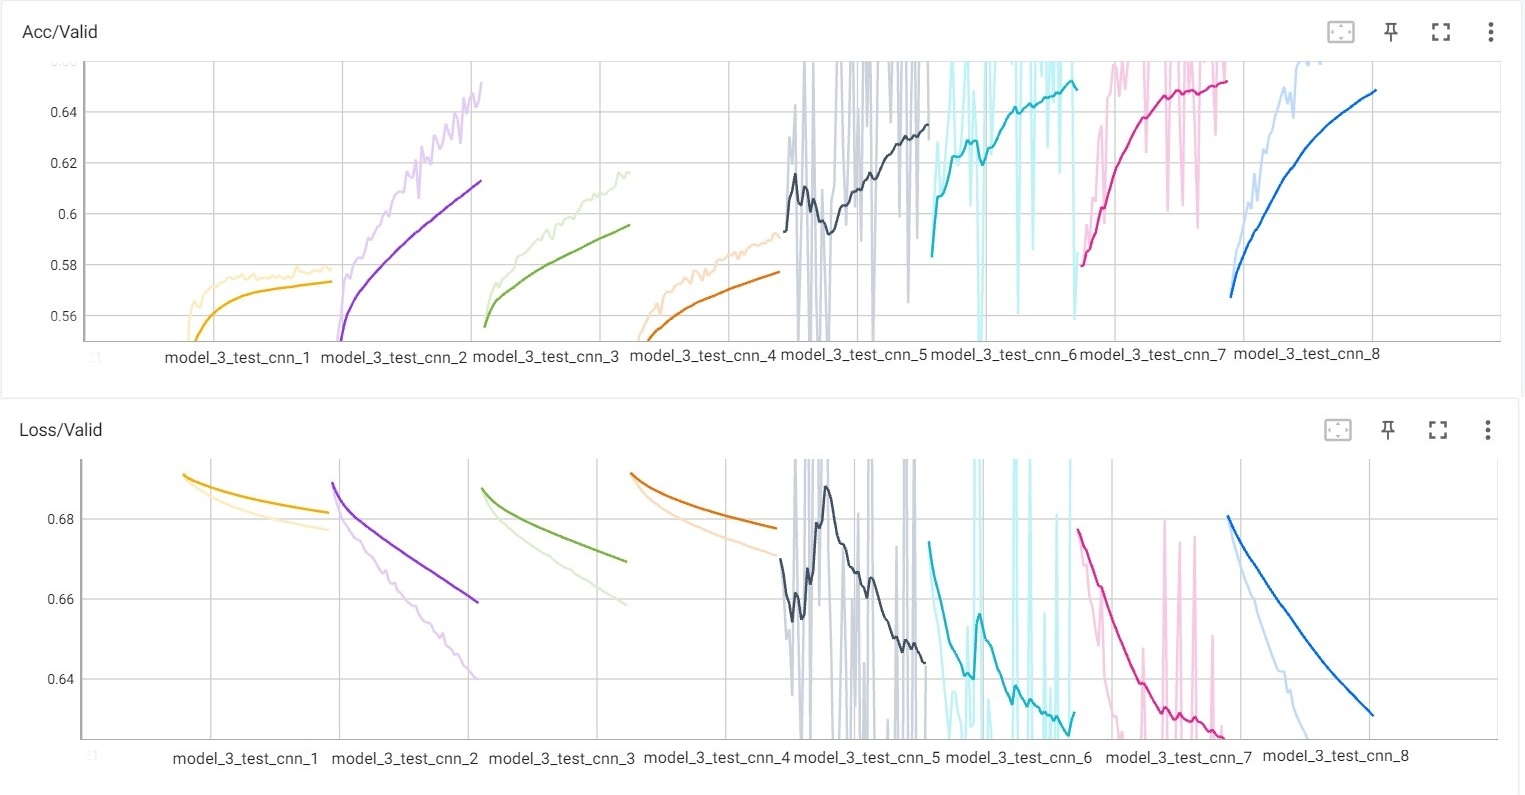
\includegraphics[width=\textwidth]{images/exp1_acc3+loss3.jpg}
        \label{fig:exp1_model3}
        \caption{Results for Model 3 at different learning rates}
    \end{figure}
\end{center}



\subsubsection{Model 4}

% Model arhitecture :
% \begin{lstlisting}[language=Python]
%     class MLP(nn.Module):
%       def __init__(self):
%         super().__init__()
%         self.layer1 = nn.Linear(768, 512)
%         self.layer2 = nn.Linear(512, 128)
%         self.layer3 = nn.Linear(128, 2)
%         self.activation = nn.ReLU()
%       def forward(self, x):
%         out = self.activation(self.layer1(x))
%         out = self.layer2(out)
%         out = self.layer3(out)
%         return out
% \end{lstlisting}

The model described in the code snippet is a multi-layer perceptron (MLP) with three hidden layers implemented using PyTorch's nn.Module class. It is similar to model 1, with the main difference consisting of it having only 3 layers instead of 3. Their dimensionality is set off at 768 and then merged at 512, 128 and 2 respectively. The results are shown in the table below:

% This MLP architecture is designed for a binary classification task. The input to the model is expected to have a size of 768.

% In the initialization method (\_\_init\_\_), the model's architecture is defined. It consists of three linear layers (self.layer1, self.layer2, and self.layer3) with 512, 128, and 2 units, respectively. Each linear layer represents a fully connected layer, where each neuron is connected to every neuron in the previous layer. The first linear layer takes the input of size 768 and outputs a tensor of size 512. The second linear layer takes the output of the previous layer (512) and outputs a tensor of size 128. Finally, the third linear layer takes the output of the second layer (128) and produces a tensor of size 2, representing the predicted class probabilities for the binary classification task.

% The ReLU activation function (self.activation) is applied between the first and second layers. ReLU (Rectified Linear Unit) is a commonly used activation function that introduces non-linearity into the model by setting negative values to zero and keeping positive values unchanged.

% In the forward method, the input x is passed through the layers of the model. First, the input is passed through the first linear layer (self.layer1) and then through the activation function (self.activation) which applies the ReLU activation element-wise. The resulting tensor is then passed through the second and third linear layers without an intermediate activation function.

% Overall, the model architecture described in the code snippet is an MLP with three hidden layers and ReLU activation function. It takes an input of size 768, processes it through the layers, and produces the final output of size 2 for the binary classification task.

\begin{center}
    \begin{figure}[!ht]
        \centering
        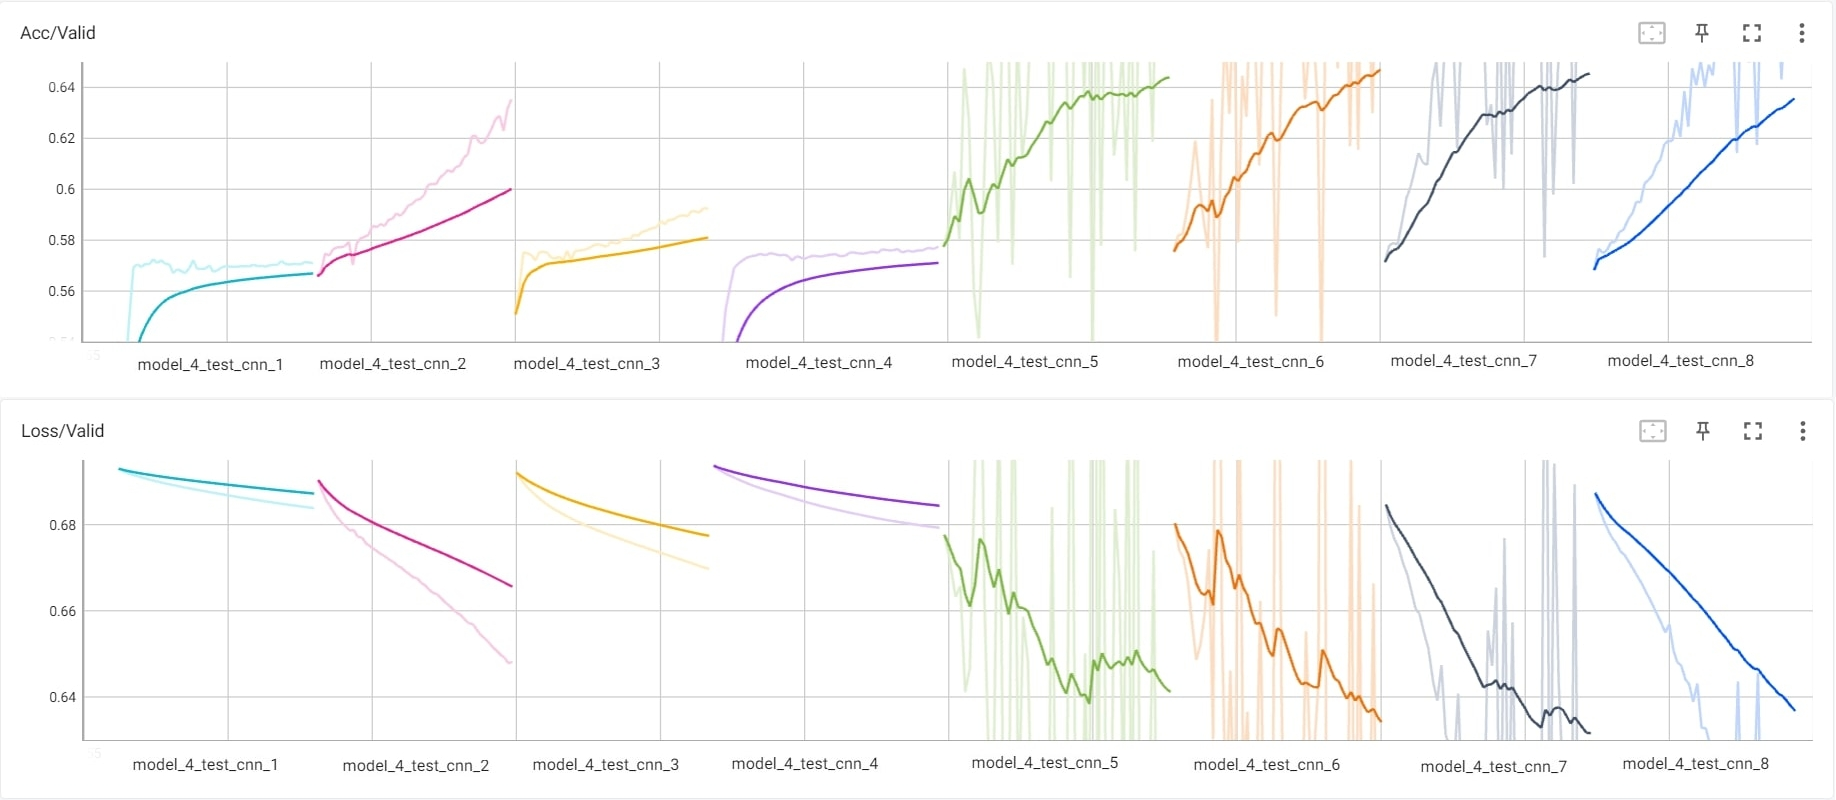
\includegraphics[width=\textwidth]{images/exp1_acc4+loss4.jpg}
        \label{fig:exp1_model4}
        \caption{Results for Model 4 at different learning rates}
    \end{figure}
\end{center}

\subsubsection{Model 5}

% Model arhitecture :
% \begin{lstlisting}[language=Python]
%     class MLP(nn.Module):
%       def __init__(self):
%         super().__init__()
%         self.layer1 = nn.MaxPool1d(3, stride=2)
%         self.layer2 = nn.Linear(383, 128)
%         self.layer3 = nn.Linear(128, 2)
%         self.activation = nn.Tanh()
%         self.drop = nn.Dropout1d(p=0.1)
%       def forward(self, x):
%         out = self.activation(self.layer1(x))
%         out = self.layer2(out)
%         out = self.drop(out)
%         out = self.layer3(out)
%         return out
% \end{lstlisting}

The model described in the code snippet is a multi-layer perceptron (MLP) with max pooling, dropout regularization, and a hyperbolic tangent activation function implemented using PyTorch's nn.Module class. Model 5 is similar to model 3. The difference consists in adding a maxpool1d layer before the first linear layer. The results are shown in the table below:

% This MLP architecture is designed for a binary classification task. The input to the model is expected to have a size that allows for max pooling.

% In the initialization method (\_\_init\_\_), the model's architecture is defined. It consists of a max pooling layer (self.layer1) with a kernel size of 3 and a stride of 2, which reduces the spatial dimensions of the input. Following the max pooling layer, there are two linear layers (self.layer2 and self.layer3) with 128 and 2 units, respectively. Each linear layer represents a fully connected layer, where each neuron is connected to every neuron in the previous layer.

% The hyperbolic tangent (Tanh) activation function (self.activation) is applied after the max pooling layer and the first linear layer. The Tanh activation function maps the input values to the range [-1, 1].

% In addition, a dropout layer with a dropout rate of 0.1 is included (self.drop). Dropout regularization randomly sets a fraction of input units to 0 during training, reducing overfitting and improving generalization.

% In the forward method, the input x is passed through the layers of the model. The input first goes through the max pooling layer (self.layer1), followed by the hyperbolic tangent activation function (self.activation). Then, the output is passed through the second linear layer (self.layer2). After that, dropout is applied to the output using self.drop. Finally, the output from the dropout layer is fed into the third linear layer (self.layer3) to produce the final output of the model.

% The output of the model represents the predicted class probabilities for a binary classification task.

% In summary, this model is an MLP with max pooling, dropout regularization, and a hyperbolic tangent activation function. The max pooling layer reduces the spatial dimensions, the dropout layer helps prevent overfitting, and the hyperbolic tangent activation function allows for non-linear transformations.

\begin{center}
    \begin{figure}[!h]
        \centering
        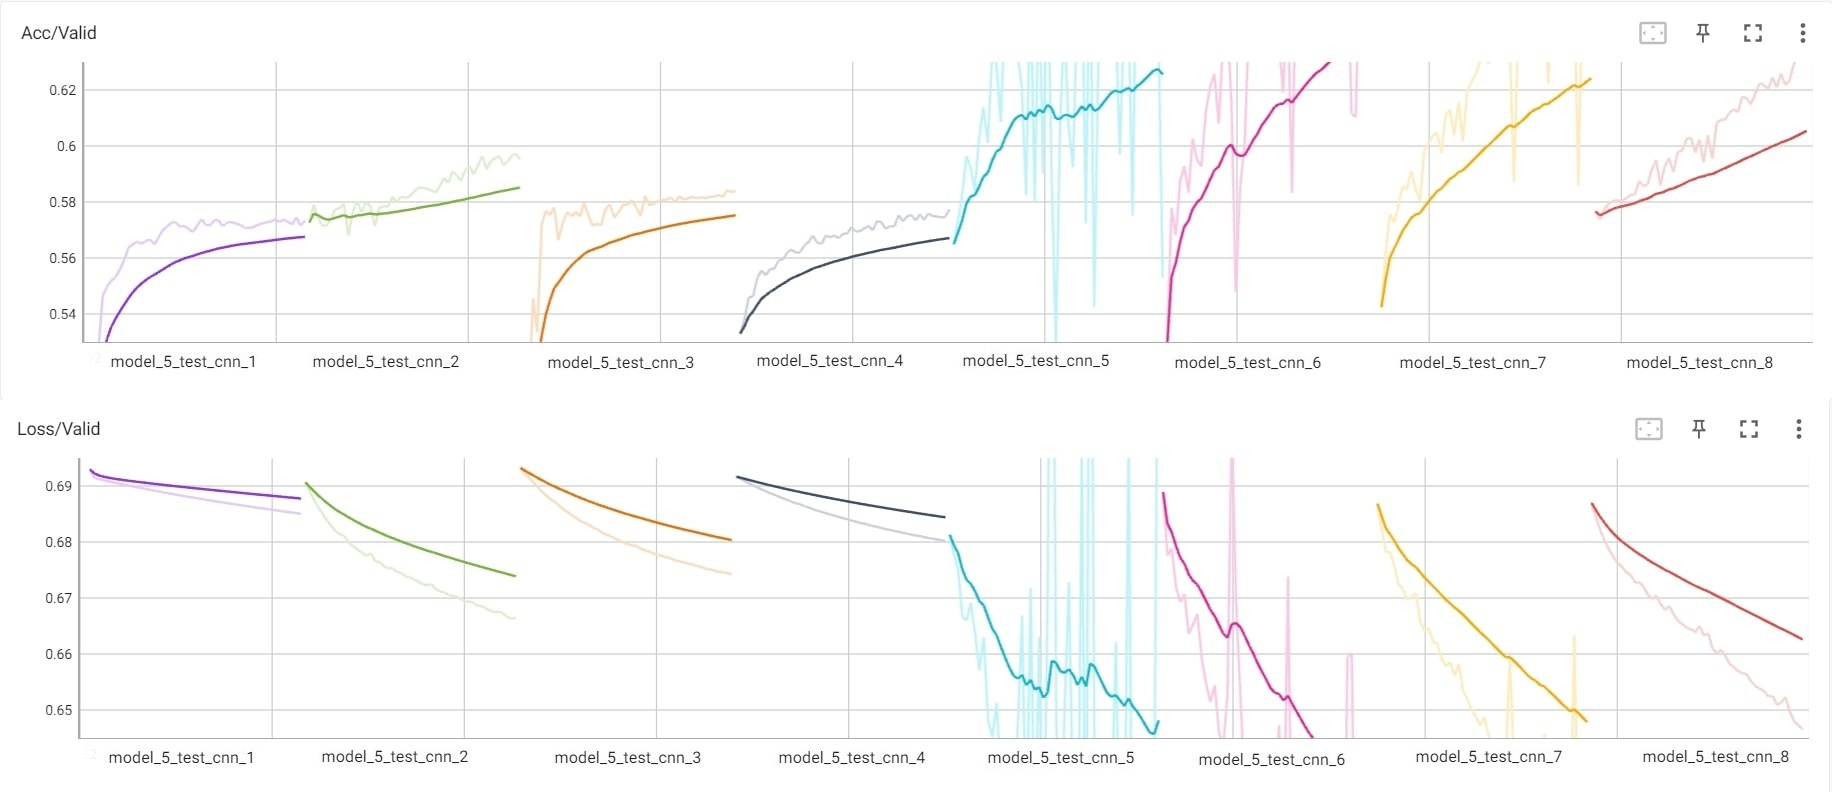
\includegraphics[width=\textwidth]{images/exp1_acc5+loss5.jpg}
        \label{fig:exp1_model5}
        \caption{Results for Model 5 at different learning rates}
    \end{figure}
\end{center}

\subsubsection{Model 6}

% Model arhitecture :
% \begin{lstlisting}[language=Python]
%     class MLP(nn.Module):
%       def __init__(self):
%         super().__init__()
%         self.layer1 = nn.MaxPool1d(3, stride=2)
%         self.layer2 = nn.Linear(383, 128)
%         self.layer3 = nn.Linear(128, 2)
%         self.activation = nn.RReLU()
%         self.drop = nn.Dropout1d(p=0.15)
%       def forward(self, x):
%         out = self.activation(self.layer1(x))
%         out = self.layer2(out)
%         out = self.drop(out)
%         out = self.layer3(out)
%         return out
% \end{lstlisting}

The model described in the code snippet is a multi-layer perceptron (MLP) with max pooling, dropout regularization, and a randomized leaky rectified linear unit (RReLU) activation function implemented using PyTorch's nn.Module class. Based on model 5 we changed the activation function from tanh to relu. Also, the dropout probability was raised from 0.1 to 0.5. The results are presented in the graph below:

% This MLP architecture is designed for a binary classification task. The input to the model is expected to have a size that allows for max pooling.

% In the initialization method (\_\_init\_\_), the model's architecture is defined. It consists of a max pooling layer (self.layer1) with a kernel size of 3 and a stride of 2, which reduces the spatial dimensions of the input. Following the max pooling layer, there are two linear layers (self.layer2 and self.layer3) with 128 and 2 units, respectively. Each linear layer represents a fully connected layer, where each neuron is connected to every neuron in the previous layer.

% The randomized leaky rectified linear unit (RReLU) activation function (self.activation) is applied after the max pooling layer and the first linear layer. RReLU is a variant of the rectified linear unit (ReLU) activation function that introduces a random component to the negative range, allowing for potential learning even when the input is negative.

% In addition, a dropout layer with a dropout rate of 0.15 is included (self.drop). Dropout regularization randomly sets a fraction of input units to 0 during training, reducing overfitting and improving generalization.

% In the forward method, the input x is passed through the layers of the model. The input first goes through the max pooling layer (self.layer1), followed by the RReLU activation function (self.activation). Then, the output is passed through the second linear layer (self.layer2). After that, dropout is applied to the output using self.drop. Finally, the output from the dropout layer is fed into the third linear layer (self.layer3) to produce the final output of the model.

% The output of the model represents the predicted class probabilities for a binary classification task.

% In summary, this model is an MLP with max pooling, dropout regularization, and a randomized leaky rectified linear unit (RReLU) activation function. The max pooling layer reduces the spatial dimensions, the dropout layer helps prevent overfitting, and the RReLU activation function introduces randomness to negative inputs, potentially aiding learning.


\begin{center}
    \begin{figure}[!h]
        \centering
        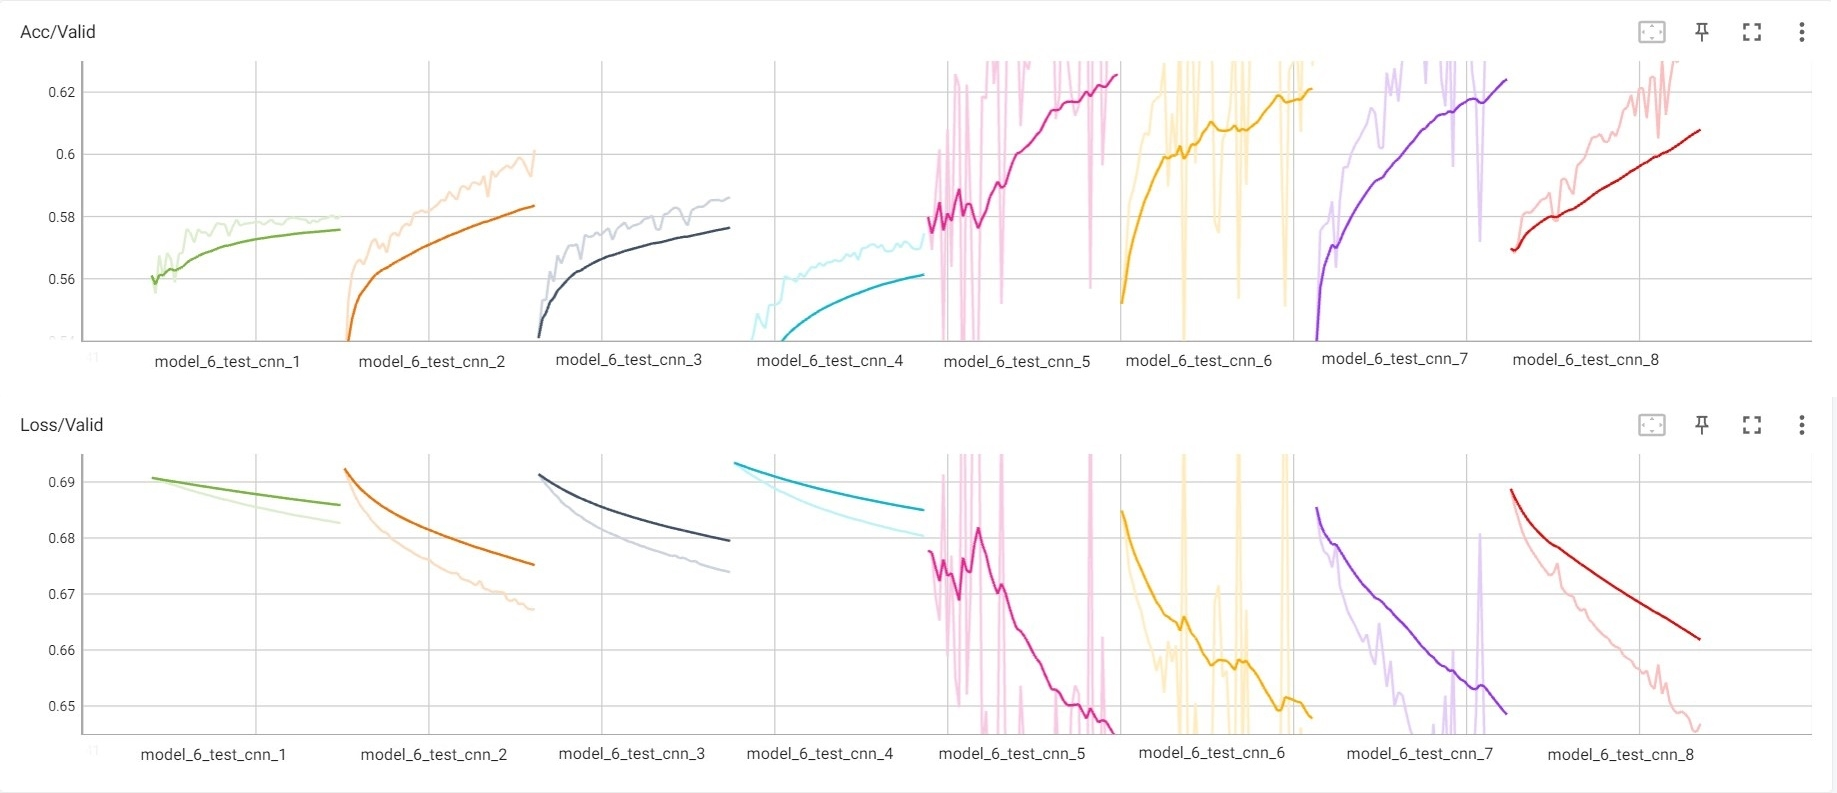
\includegraphics[width=\textwidth]{images/exp1_acc6+loss6.jpg}
        \label{fig:exp1_model6}
        \caption{Results for Model 6 at different learning rates}
    \end{figure}
\end{center}


\subsubsection{Comparation}
\begin{center}
    \begin{tabular}{|p{3cm}||p{3cm}|p{3cm}|  }
     % \hline
     % \multicolumn{3}{|c|}{BERT fine-tunning results} \\
     \hline
    Model number	& Accuracy & Loss \\
     \hline
    Model 1 & 71.07\% & 0.5611\\
    \textbf{Model 2} & \textbf{71.23}\% & 0.5691\\
    \textbf{Model 3} & \textbf{71.4}\% & 0.5682\\
    \textbf{Model 4} & \textbf{71.42}\% & 0.5611\\
    Model 5 & 68.58\% & 0.5994\\
    Model 6 & 69.03\% & 0.6034\\
     \hline
    \end{tabular}
    \captionof{table}{BERT fine-tunning results: Experiment 1}
\end{center}

As already noticed, models 2, 3 and 4 had high accuracy, so we will use them to do fine tuning when we retrain the BERT model as well.

\begin{center}
    \begin{figure}[!h]
        \centering
        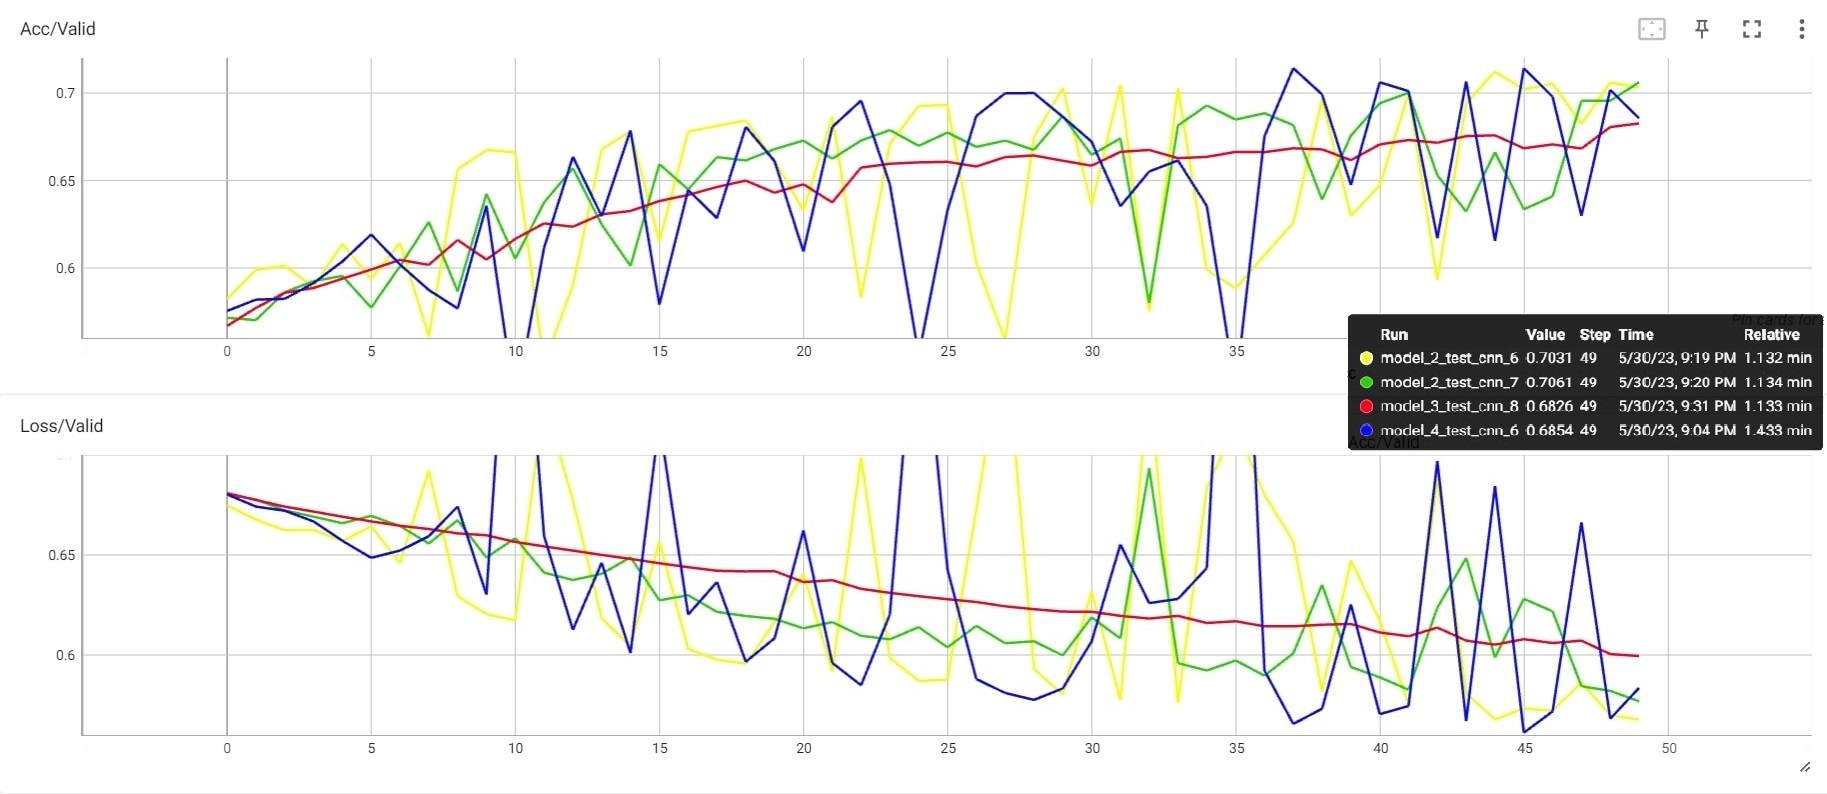
\includegraphics[width=\textwidth]{images/exp1_hiperparametrizare.jpg}
        \label{fig:exp1_hiperm}
        \caption{Results for Model 2, 3 and 4}
    \end{figure}
\end{center}

\subsection{Experiment 2}

In experiment 2, I took Models 2, 3 and 4 and redefined the Neural Network class to retrain with BERT. The learning rate took the values: $4*10^{-5}, 2*10^{-5}$. The batch size was kept at 32.

\subsubsection{Model 2}

Code for this model defines a PyTorch module called MLP that incorporates a BERT model as part of its architecture. The BERT model is passed as a parameter mod to the \_\_init\_\_ method. Here's a breakdown of the model's components and functionality:

\begin{itemize}
    \item self.bert = mod: This line assigns the BERT model received in the mod variable to the self.bert attribute of the MLP class.
    \item self.layer1 = nn.Linear(768, 256): This creates a linear layer with an input size of 768 and an output size of 256. It is the first layer after the BERT model.
    \item self.layer2 = nn.Linear(256, 2): This creates another linear layer with an input size of 256 and an output size of 2. It is the second and final layer of the MLP.
    \item self.activation = nn.ReLU(): This defines the activation function to be applied after the first linear layer. In this case, it uses the Rectified Linear Unit (ReLU) activation function.
    \item self.drop = nn.Dropout1d(p=0.1): This creates a dropout layer with a dropout rate of 0.1. 
\end{itemize}

The forward method of the MLP class implements the forward pass of the model. Here's a breakdown of its steps:
\begin{itemize}
    \item out = self.bert(ids, attention\_mask=mask, token\_type\_ids=token\_type\_ids) \newline ['pooler\_output']: This line applies the BERT model to the input ids, mask, and token\_type\_ids. It retrieves the 'pooler\_output' from the BERT model's output dictionary. The 'pooler\_output' typically represents a fixed-size representation of the entire input sequence.

    \item out = self.activation(out): tensor is passed through the activation function. In this case, it uses the ReLU activation function. This line is tested both : commented, which means that BERT output is not activated - Model 2A, and not commented, which means that BERT output is activated - Model 2B.

    \item out = self.activation(self.layer1(out)): The out tensor is passed through the first linear layer and then activated using the ReLU activation function.

    \item out = self.drop(out): Dropout is applied to the output of the first linear layer.

    \item out = self.layer2(out): The output from the dropout layer is passed through the second linear layer.

    \item return out: The final output of the MLP is returned.
\end{itemize}

In summary, this MLP class integrates a BERT model as a component of its architecture and applies a two-layer feed-forward neural network on top of the BERT output to perform a specific task, which is not evident from the provided code.

\begin{center}
    \begin{figure}[!h]
        \centering
        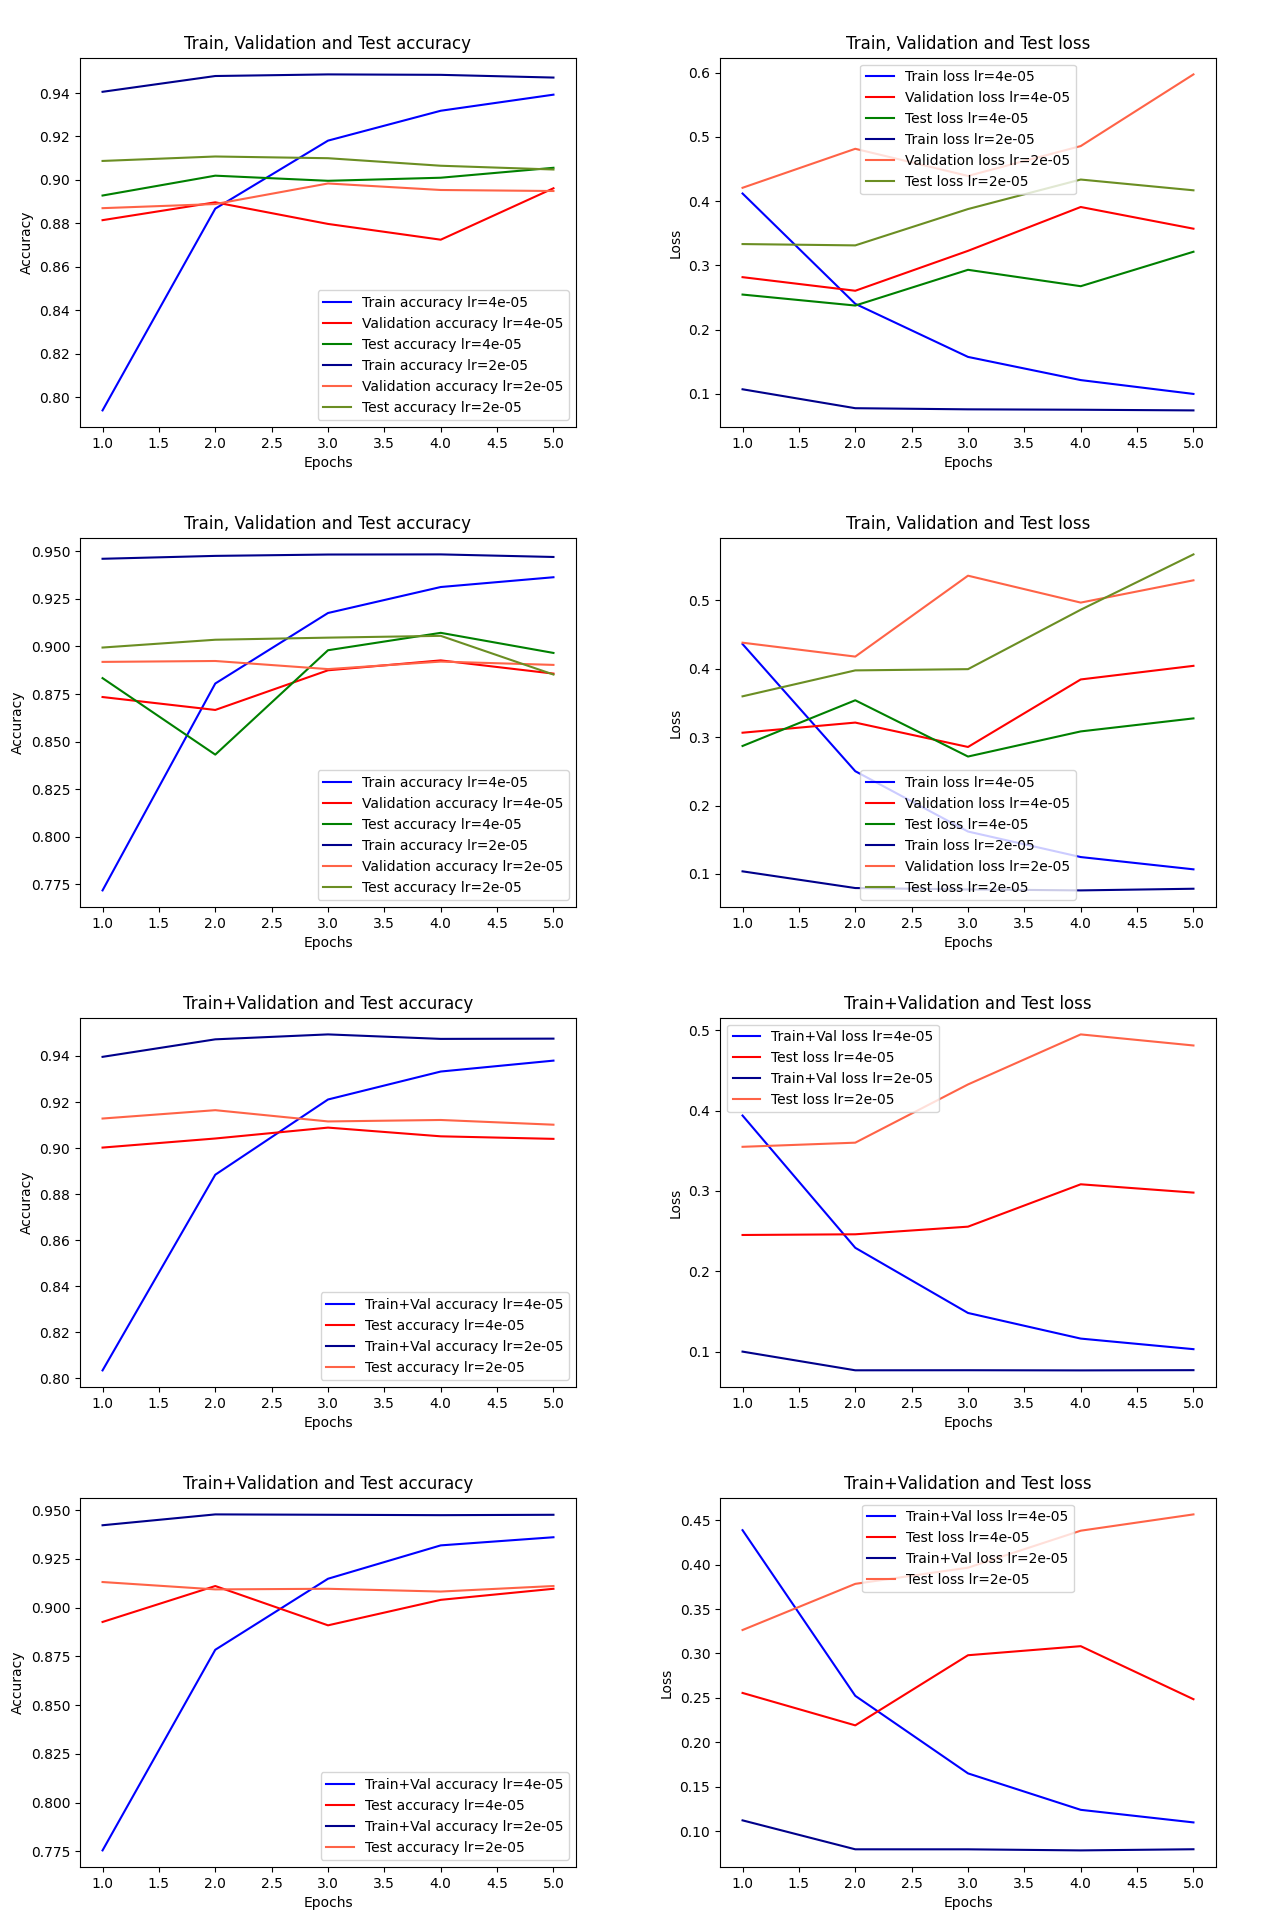
\includegraphics[width=0.8\textwidth]{images/ger_model1_vertical.png}
        \label{fig:ger_model1}
        \caption{Results for Model 2 with and without BERT activation. Tested on Validation(top half) and on Test(bottom half)}
    \end{figure}
\end{center}


\subsubsection{Model 3}

Code for this model defines a PyTorch module called MLP that incorporates a BERT model as part of its architecture. The BERT model is passed as a parameter mod to the \_\_init\_\_ method. Here's a breakdown of the model's components and functionality:

\begin{itemize}
    \item self.bert = mod: This line assigns the BERT model received in the mod variable to the self.bert attribute of the MLP class.

    \item self.layer1 = nn.Linear(768, 256): This creates a linear layer with an input size of 768 and an output size of 256. It is the first layer after the BERT model.

    \item self.layer2 = nn.Linear(256, 2): This creates another linear layer with an input size of 256 and an output size of 2. It is the second and final layer of the MLP.

    \item self.activation = nn.Tanh(): This defines the activation function to be applied after the BERT output and the first linear layer. In this case, it uses the hyperbolic tangent (Tanh) activation function.

    \item self.drop = nn.Dropout1d(p=0.1): This creates a dropout layer with a dropout rate of 0.1. Dropout is applied to prevent wrongly classifying certain data as important by unsystematically positioning a fraction of the input elements to zero in the training process.
    
\end{itemize}


The forward method of the MLP class implements the forward pass of the model. Here's a breakdown of its steps:

\begin{itemize}
    \item out = self.bert(ids, attention\_mask=mask, token\_type\_ids=token\_type\_ids) \newline ['pooler\_output']: This line applies the BERT model to the input ids, mask, and token\_type\_ids. It retrieves the 'pooler\_output' from the BERT model's output dictionary. The 'pooler\_output' typically represents a fixed-size representation of the entire input sequence.

    \item out = self.activation(out): The out tensor is passed through the activation function, which is the hyperbolic tangent (Tanh) in this case. This line is tested both : commented, which means that BERT output is not activated - Model 3A, and not commented, which means that BERT output is activated - Model 3B.

    \item out = self.activation(self.layer1(out)): The output from the previous activation function is passed through the first linear layer and then activated using the Tanh activation function again.

    \item out = self.drop(out): Dropout is applied to the output of the first linear layer.

    \item out = self.layer2(out): The output from the dropout layer is passed through the second linear layer.

    \item return out: The final output of the MLP is returned.
\end{itemize}

In summary, this MLP class integrates a BERT model as a component of its architecture and applies a two-layer feed-forward neural network on top of the BERT output. The activation function used in this model is the hyperbolic tangent (Tanh). Dropout is applied to the output of the first linear layer to prevent overfitting.

\begin{center}
    \begin{figure}[!h]
        \centering
        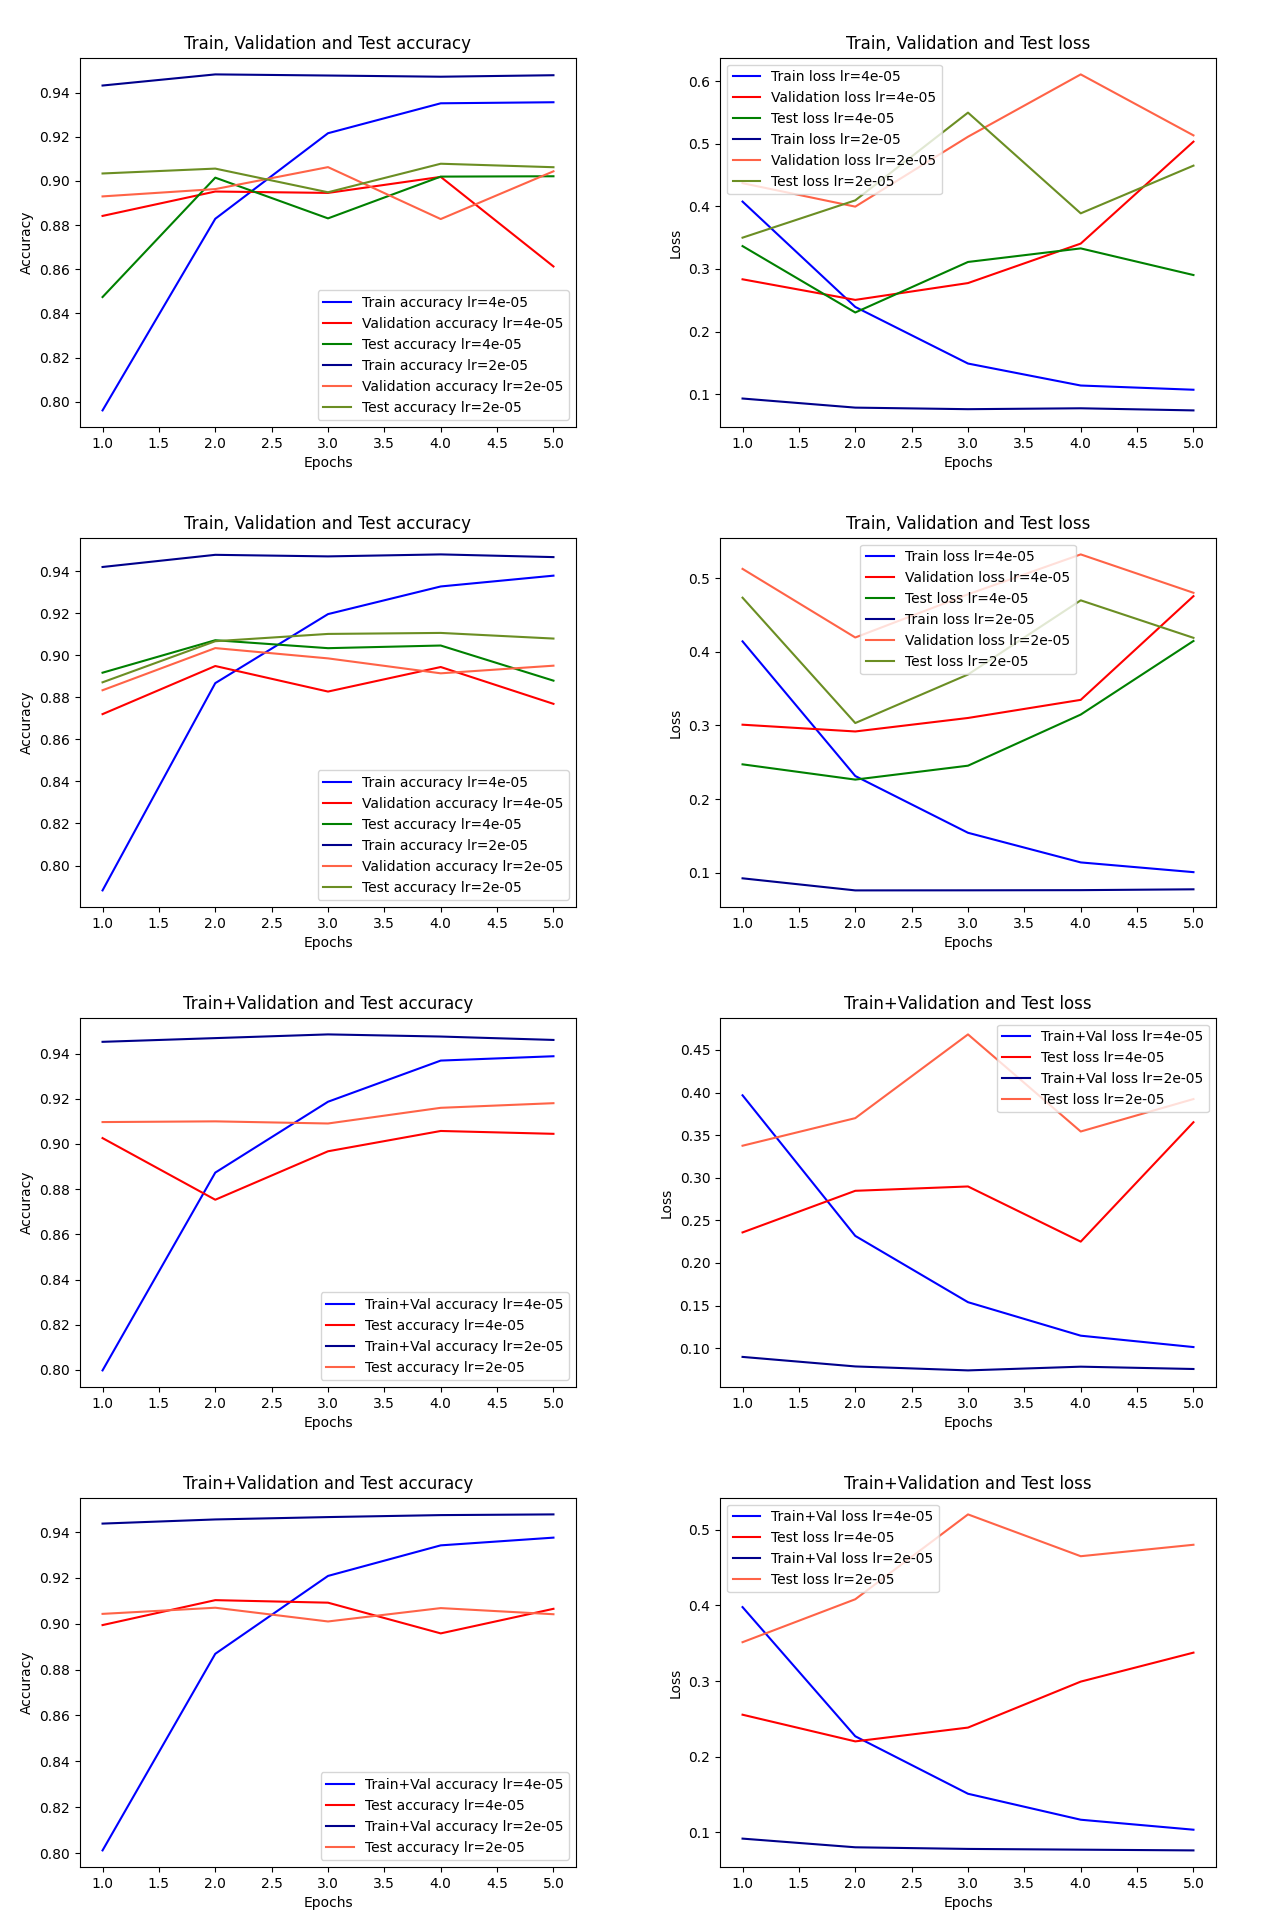
\includegraphics[width=0.8\textwidth]{images/ger_model2_vertical.png}
        \label{fig:ger_model2}
        \caption{Results for Model 3 with and without BERT activation. Tested on Validation(top half) and on Test(bottom half)}
    \end{figure}
\end{center}


\subsubsection{Model 4}

Code for this model defines a PyTorch module called MLP that incorporates a BERT model as part of its architecture. The BERT model is passed as a parameter mod to the \_\_init\_\_ method. Here's a breakdown of the model's components and functionality:

\begin{itemize}
    \item self.bert = mod: This line assigns the BERT model received in the mod variable to the self.bert attribute of the MLP class.

    \item self.layer1 = nn.Linear(768, 512): This creates a linear layer with an input size of 768 (the output size of the BERT model) and an output size of 512.

    \item self.layer2 = nn.Linear(512, 128): This creates another linear layer with an input size of 512 and an output size of 128.

    \item self.layer3 = nn.Linear(128, 2): This creates the final linear layer with an input size of 128 and an output size of 2.

    \item self.activation = nn.ReLU(): This defines the activation function to be applied after each linear layer. In this case, it uses the Rectified Linear Unit (ReLU) activation function.
\end{itemize}

The forward method of the MLP class implements the forward pass of the model. Here's a breakdown of its steps:

\begin{itemize}
    \item out = self.bert(ids, attention\_mask=mask, token\_type\_ids=token\_type\_ids) \newline ['pooler\_output']: This line applies the BERT model to the input ids, mask, and token\_type\_ids. It retrieves the 'pooler\_output' from the BERT model's output dictionary. The 'pooler\_output' typically represents a fixed-size representation of the entire input sequence.

    \item out = self.activation(out): The out tensor is passed through the activation function, which is the Rectified Linear Unit (ReLU) in this case. This line is tested both : commented, which means that BERT output is not activated - Model 4A, and not commented, which means that BERT output is activated - Model 4B.

    \item out = self.activation(self.layer1(out)): The output from the previous activation function is passed through the first linear layer and then activated using the ReLU activation function again.

    \item out = self.layer2(out): The output from the previous layer is passed through the second linear layer.

    \item out = self.layer3(out): The output from the previous layer is passed through the final linear layer.

    \item return out: The final output of the MLP is returned.
\end{itemize}

In summary, this MLP class integrates a BERT model as a component of its architecture and applies a three-layer feed-forward neural network on top of the BERT output. The activation function used between the linear layers is the Rectified Linear Unit (ReLU). The output of the last linear layer is returned as the final output of the MLP.

\begin{center}
    \begin{figure}[!h]
        \centering
        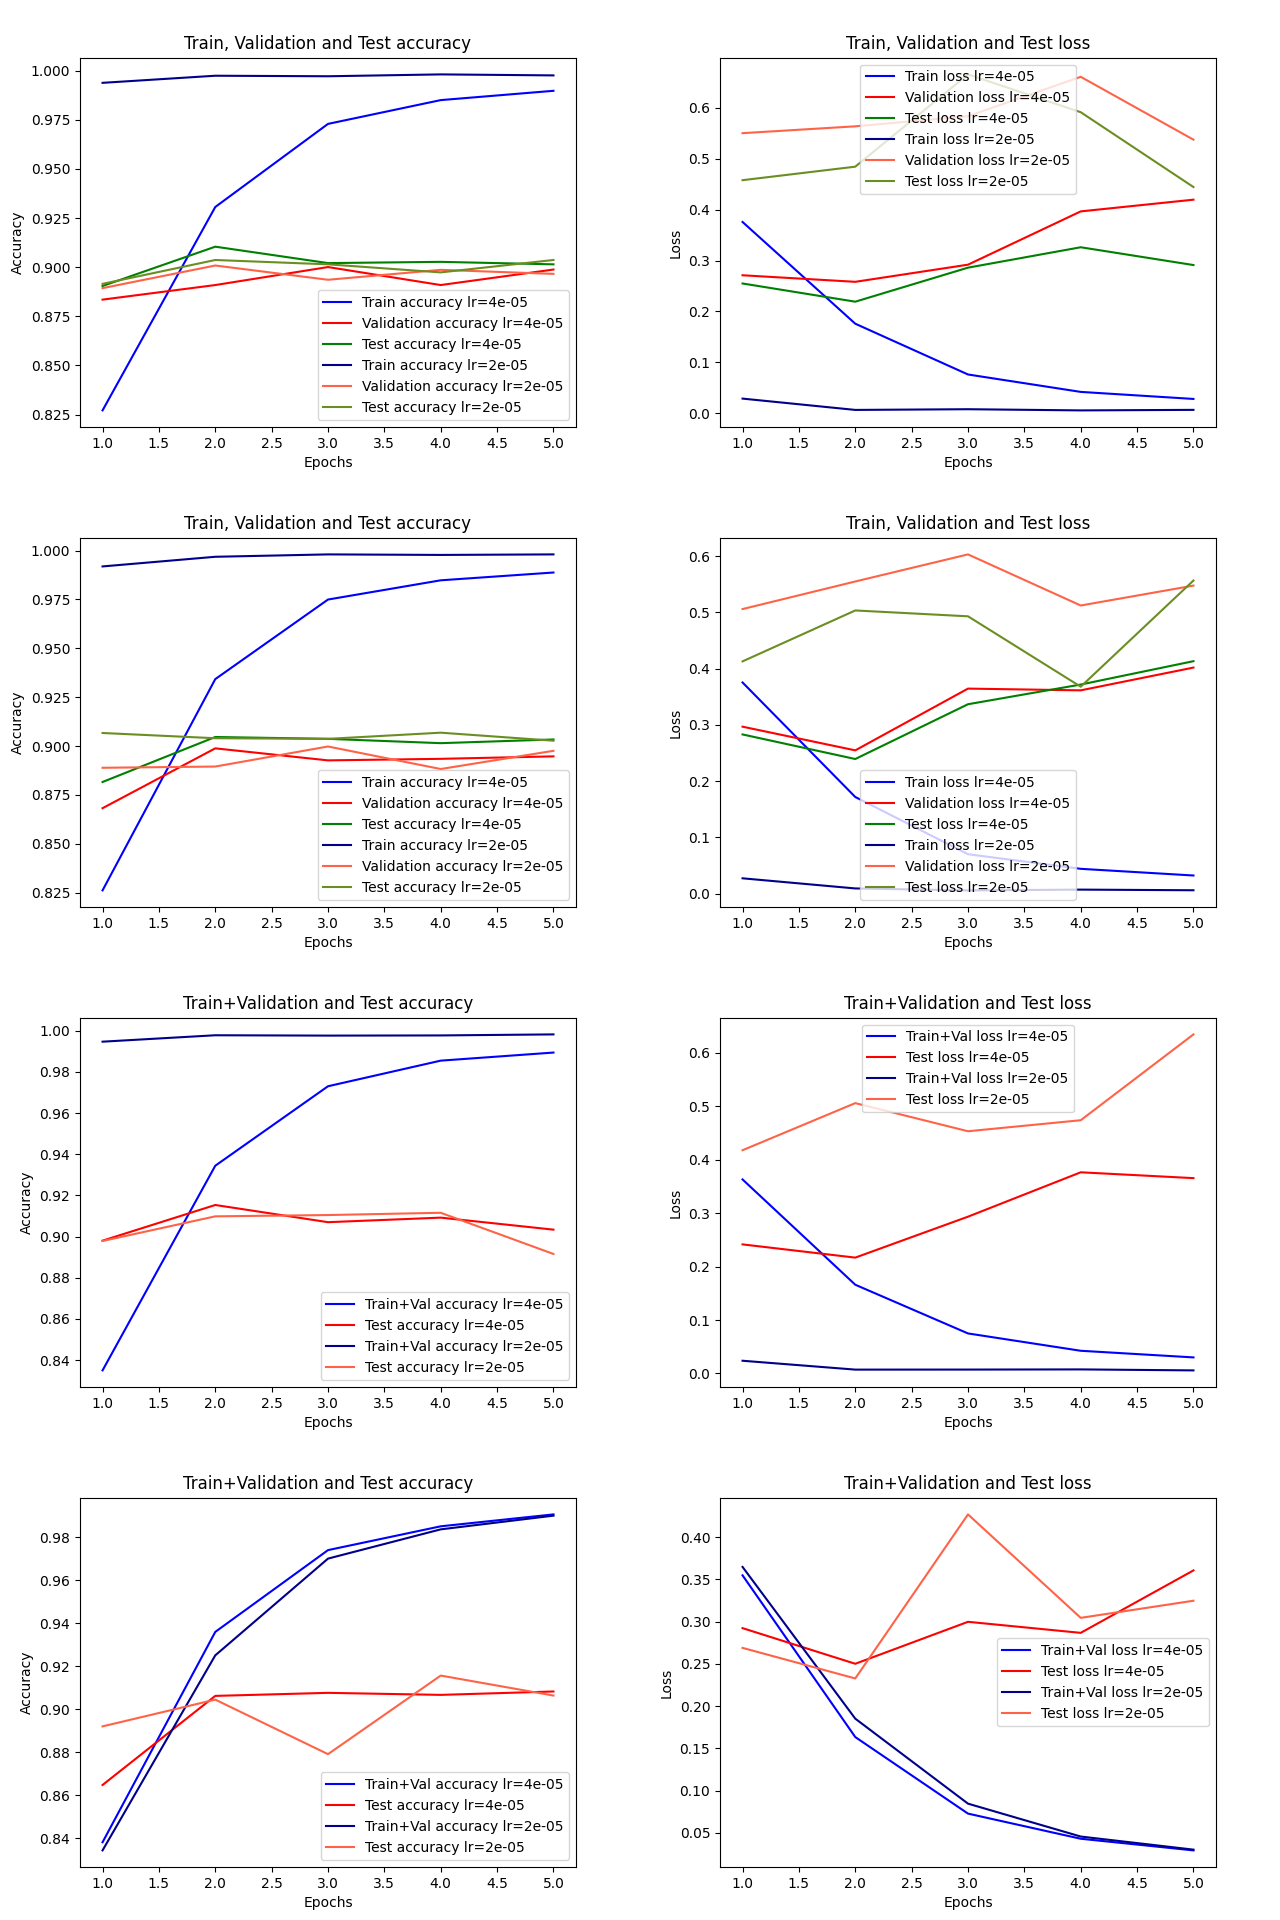
\includegraphics[width=0.8\textwidth]{images/ger_model3_vertical.png}
        \label{fig:ger_model3}
        \caption{Results for Model 4 with and without BERT activation. Tested on Validation(top half) and on Test(bottom half)}
    \end{figure}
\end{center}


\chapter{Conclusion}
\label{chap:conclusion}

\section{Key Results}

This section provides a concise overview of the key discoveries and insights gained from the study.

Throughout the research, the effectiveness of employing large language models in translationese classification was investigated. The results demonstrated that these models, with their ability to capture complex linguistic patterns, can be highly successful in identifying and classifying translationese. The performance of the models surpassed that of traditional machine learning approaches, indicating their potential for advancing translation studies.

\begin{center}
    \begin{tabular}{|p{2.5cm}||p{2.5cm}|p{2.5cm}|p{2.5cm}|p{2.5cm}|  }
     % \hline
     % \multicolumn{5}{|c|}{BERT fine-tunning results} \\
     \hline
    Model no.	& Acc on Train	& Loss on Train & Acc on Test & Loss on Test\\
     \hline
     \multicolumn{5}{|c|}{DE-EN dataset} \\
     \hline
    Model 2-A&  94.935\%  &  0.103  &  91.646\%  &  0.36 \\
    Model 2-B&  94.785\%  &  0.11  &  91.315\%  &  0.326 \\
    Model 3-A&  94.846\%  &  0.101  &  91.803\%  &  0.392 \\
    Model 3-B&  94.771\%  &  0.103  &  91.031\%  &  0.408 \\
    Model 4-A&  99.825\%  &  0.03  &  91.535\%  &  0.474 \\
    Model 4-B&  99.067\%  &  0.03  &  91.567\%  &  0.361 \\
     \hline
     \multicolumn{5}{|c|}{ES-EN dataset} \\
     \hline
    Model 2-A&  95.097\%  &  0.102  &  91.992\%  &  0.325 \\
    Model 2-B&  95.005\%  &  0.1  &  92.04\%  &  0.384 \\
    Model 3-A&  94.963\%  &  0.102  &  92.055\%  &  0.409 \\
    Model 3-B&  94.944\%  &  0.099  &  92.323\%  &  0.365 \\
    Model 4-A&  99.833\%  &  0.03  &  91.992\%  &  0.404 \\
    Model 4-B&  99.805\%  &  0.028  &  92.229\%  &  0.358 \\
     \hline
     \multicolumn{5}{|c|}{A: BERT not activated, B: BERT activated} \\
     \hline
    \end{tabular}
    \captionof{table}{BERT results: Experiment 2}
\end{center}

The study highlighted the importance of feature extraction from the language model, such as token-level probabilities and contextual embeddings. These features played a vital role in distinguishing between translationese and native language writing, capturing distinct linguistic traits present in translated texts.

Additionally, the research compared different classification models and found that neural networks, particularly those incorporating BERT architectures, succeeded in the highest classification accuracy. This observation further emphasized the effectiveness of neural network models in capturing intricate linguistic patterns associated with translationese.

Furthermore, the study showcased the strength and universal applicability of information from the large language model-based approach. Our models exhibited consistent performance across various language pairs and translation domains, indicating their potential for application in diverse translation scenarios.

\vspace{0.2cm}

\begin{center}
    \begin{tabular}{|p{2.5cm}||p{2.5cm}|p{2.5cm}|  }
     % \hline
     % \multicolumn{3}{|c|}{Compared results} \\
     \hline
    Dataset	& Model & Accuracy \\
     \hline
     \hline
    DE-EN&  $BERT^{*}$  &  \textbf{92.4}\%\\
    DE-EN&  Model 3-A  &  91.8\%  \\
    \hline
    \hline
    ES-EN&  $BERT^{*}$  &  91.4\%\\
    ES-EN&  Model 3-B  &  \textbf{92.32}\%  \\
     \hline
     \multicolumn{3}{|c|}{$BERT^{*}$: BERT best result from paper \cite{mainpaper}} \\
     \hline
    \end{tabular}
    \captionof{table}{Compared results}
\end{center}

$BERT^{*}$ is the model used in the paper \cite{mainpaper}. This model was created by combining bert-base-uncased and fine-tuned using the simpletransformers\footnote{github.com/ThilinaRajapakse/
simpletransformers} library.

\section{Constraints}

While the research achieved promising results, it is essential to acknowledge the limitations encountered during the study. One potential limitation is the reliance on pre-existing large language models, such as GPT-3, which may present their own biases or limitations. The generalizability of the findings should be considered in light of the specific language model used.

Another limitation consists of the requirement for extensive computational resources to train and fine-tune the language model. The computational requirements may limit the accessibility and scalability of this approach, particularly for researchers with limited resources.

Moreover, the study focused on the classification of translationese but did not extensively explore the underlying causes or implications of translationese patterns. Further research is necessary to delve deeper into the specific linguistic phenomena and translation strategies associated with translationese.

\section{Practic Applications of our model}

The paper "Using Large Language Models in Translationese Classification" explores the effectiveness of employing large language models, specifically BERT, for detecting English translationese. The findings from this study have several practical applications that can benefit various stakeholders in the field of translation and language processing. Here are some practical applications of a BERT model trained to detect English translationese classification based on the research:

\begin{enumerate}
    \item Translation Quality Assessment: Large language models trained to detect translationese can be utilized as an objective tool for translated-text quality assessment. By analyzing the possible presence and extent of translationese patterns, translation agencies, professional translators, and language service providers can gain valuable insights into the stylistic and linguistic characteristics of translations, allowing them to identify areas for improvement and enhance the overall quality of translated content.

    \item Translator Training and Feedback: BERT models trained for translationese classification can serve as an educational tool for translator training programs. By providing real-time feedback on translation outputs, these models can help aspiring translators understand the challenges associated with translationese and develop strategies to avoid or mitigate its occurrence. This can lead to more accurate and culturally appropriate translations.

    \item Translation Memory Optimization: Translation memory (TM) systems store previously translated segments to aid translators in their work. By incorporating a BERT model trained to detect translationese into TM systems, translators can receive suggestions or warnings when translationese patterns are detected in segments. This can help maintain consistency and ensure that previous translation choices are appropriately adapted to the context.

    \item Machine Translation Improvement: Large language models trained for translationese classification can be integrated into machine translation (MT) systems to enhance their output quality. By identifying translationese patterns in the output of MT systems, improvements can be made to reduce the occurrence of unnatural or non-idiomatic translations. This can contribute to the development of more accurate and fluent machine translation systems.

    \item Corpus Analysis and Comparative Studies: Researchers and linguists can utilize BERT models trained for translationese classification to conduct corpus analyses and comparative studies between translations and original texts. These models can aid in uncovering and understanding the specific linguistic features, shifts in writing style, or lexical choices that characterize translationese. Such analyses can provide valuable insights into cross-linguistic phenomena, translation strategies, and intercultural communication.

    \item Style Guide Development: BERT models trained to detect translationese can assist in the development of style guides for translators and localization teams. By identifying and documenting translationese patterns specific to different language pairs or domains, style guides can provide guidelines for producing more natural and target language-oriented translations, ensuring consistency and coherence in the translated content.

\end{enumerate}

Overall, the practical applications of a BERT model trained to detect English translationese classification are diverse and can contribute to improving translation quality, translator training, machine translation systems, and linguistic research. By leveraging large language models in this manner, the field of translation and language processing can advance, benefiting both professionals and end-users in achieving more accurate and fluent translations.


\section{Future Research Directions}

The conclusions we can draw at the end of this translationese-focused research, are indicative of some of the key points that should be taken into consideration. Therefore, we put forward the following suggestions:

\begin{enumerate}
    \item Investigation of Translation Strategies: Further exploration of the translation strategies employed by translators that lead to the emergence of translationese patterns could provide valuable insights into cross-linguistic phenomena. Understanding these strategies can contribute to the development of more sophisticated translation models.

    \item Cross-Linguistic Analysis: Extending the study to include a broader range of languages and language pairs can help uncover language-specific characteristics and identify common translationese patterns across different linguistic backgrounds.

    \item Multimodal Translationese Classification: Investigating the application of large language models in multimodal translationese classification, where both textual and visual elements are considered, can provide a more comprehensive understanding of translationese across different modalities.

    \item Addressing Ethical Concerns: As LLMs continue to grow and expand, ethical considerations become crucial. Future research should tackle diagnosis bias worries, fairness, and more importantly, transparency in translationese classification to ensure responsible and equitable use of these models.

    \item Using bigger models: For example, this paper is used bert-base-uncased which has 110M parameters. For future work, we may want to use bert-large-uncased which has 340M parameters and may be better to classify translationese

\end{enumerate}

By pursuing these future research directions, the field of translation studies can further leverage the capabilities of large language models and advance our  extended comprehension of translationese, ultimately benefiting translation professionals and improving cross-linguistic communication.


\nocite{*}
\printbibliography[heading=bibintoc]

\end{document}